\documentclass[parskip=full]{scrartcl}

\pdfoutput=1

\title{Geometric SMOTE \\ \LARGE{A geometrically enhanced drop-in replacement for SMOTE}}

\author{
	Georgios Douzas\(^{1}\), Fernando Bacao\(^{1*}\)
	\\
	\small{\(^{1}\)NOVA Information Management School, Universidade Nova de Lisboa}
	\\
	\small{*Corresponding Author}
	\\
	\\
	\small{Postal Address: NOVA Information Management School, Campus de Campolide, 1070-312 Lisboa, Portugal}
	\\
	\small{Telephone: +351 21 382 8610}
}

\usepackage{breakcites}
\usepackage{float}
\usepackage{graphicx}
\usepackage{geometry}
\geometry{
	a4paper,
	total={170mm,257mm},
	left=18mm,
	right=18mm,
	top=8mm,
}
\usepackage{amsmath}
\newcommand{\inlineeqnum}{\refstepcounter{equation}~~\mbox{(\theequation)}}
\usepackage{enumitem}
\usepackage[ruled,vlined]{algorithm2e}
\usepackage{booktabs}
\usepackage{pgfplotstable}
\usepackage{longtable}
\usepackage{tabu}
\usepackage{hyperref}
\date{}



\begin{document}

\maketitle

\begin{abstract}
Classification of imbalanced datasets is a challenging task for standard algorithms. Although many methods exist to address this problem in different ways, generating artificial data for the minority class is a more general approach compared to algorithmic modifications. SMOTE algorithm, as well as any other oversampling method based on the SMOTE mechanism, generates synthetic samples along line segments that join minority class instances. In this paper we propose Geometric SMOTE (G-SMOTE) as a enhancement of the SMOTE data generation mechanism. G-SMOTE generates synthetic samples in a geometric region of the input space, around each selected minority instance. While in the basic configuration this region is a hyper-sphere, G-SMOTE allows its deformation to a hyper-spheroid. The performance of G-SMOTE is compared against SMOTE as well as baseline methods. We present empirical results that show a significant improvement in the quality of the generated data when G-SMOTE is used as an oversampling algorithm. An implementation of G-SMOTE is made available in the Python programming language.
\end{abstract}

\section{Introduction}
Learning from imbalanced data is a non trivial and important problem for the research community and the industry practitioners \cite{Chawla2003}. An imbalanced learning problem is defined as a classification task for binary or multi-class datasets where a significant asymmetry exists between the number of instances for the various classes. The dominant class is called the majority class while the rest of the classes are called the minority classes \cite{Chawla2003}. The Imbalance Ratio (IR), defined as the ratio between the majority class and each of the minority classes, depends on the type of application and for binary problems values between 100 and 100.000 have been observed \cite{Chawla2002}, \cite{Barua2014}.

The imbalance learning problem can be found in numerous practical domains, such as chemical and biochemical engineering, financial management, information technology, security, business, agriculture or emergency management, for a more in depth review the reader is referred to (Haixiang et al., 2017). Standard learning methods induce a bias in favor of the majority class during training. This happens because the minority classes contribute less to the minimization of the objective function, defined often as the classification accuracy. Additionally, the distinction between noisy and minority class instances is frequently difficult. As a result the performance of the classifiers, evaluated on metrics suitable for imbalanced data, is low. It is also important to consider that the costs of misclassifying the minority class are frequently much higher than the costs of misclassification of the majority class  \cite{Domingos1999}, \cite{Ting2002}. Diseases screening tests are a typical situation in in which false negatives involve a much higher cost than the false positives. Therefore, fundamentally the class imbalance challenge is to propose smart and simple ways is to improve the accuracy of classifiers for the minority class.

We can classify the approaches to deal with class imbalance into three main groups \cite{Fernandez2013}. The first consists in the modification or creation of algorithms that reinforce the learning towards the minority class. The second is the application of cost-sensitive methods to minimize higher cost errors. The last and more general approach involves the modification at the data level by re-balancing the class distribution. This is usually done through the use of undersampling, oversampling or hybrid methods.

Our focus in this paper is oversampling techniques, which result in the generation of artificial data for the minority class. Synthetic Minority Oversampling Technique (SMOTE) \cite{Chawla2002} is the most popular algorithm in this category. SMOTE can be decomposed into two parts: a set of selection rules for the minority class instances and a data generation mechanism once these samples are selected. Specifically, the selection phase constitutes of a process that repeatedly identifies one minority class sample and a random minority class k-nearest neighbor of it while the data generation mechanism creates synthetic examples along the line segment that joins them. Most existing variations of the SMOTE algorithm modify the selection phase by imposing a set of heuristic rules. Contrary to this, the method proposed in this paper, G-SMOTE, substitutes the data generation mechanism by defining a flexible geometric region around each minority class instance. Then synthetic instances are generated inside the boundaries of the region which are controlled by an appropriate parametrization of the algorithm.

For the evaluation of G-SMOTE as an oversampling method an experimental analysis is performed. The selected imbalanced datasets are publicly available from the UCI \cite{Lichman2013} and KEEL \cite{Alcala-Fdez2011} repositories. In order to test the performance of the algorithm on more extreme cases of imbalance, undersampled modifications of the aforementioned datasets as well as simulated binary class imbalanced data are provided in a total of 69 datasets. Since this work aims to show that G-SMOTE is an enhanced generalization of SMOTE, the experimental procedure includes a comparison between the two algorithms using 4 classifiers and 3 appropriate evaluation metrics. Additionally, applying no oversampling and Random Oversampling are included as baseline methods.

The sections in the paper are organized as follows. In section 2, an overview of related previous works and existing sampling methods is given. In Section 3, the motivation for G-SMOTE is presented, while section 4 describes the proposed method in detail. The experimental results as well as conclusions from their analysis are presented in section 5.

\section{Related work}

In this section we provide a brief review of the most popular oversampling methods. The reader interested in undersampling and hybrid methods is referred to  \cite{Galar2012}, \cite{Chawla2005} and \cite{Fernandez2018}. The fundamental idea of oversampling methods consists in the generation of synthetic examples for the minority class, which should then be added to the training set. The simplest approach, Random Oversampling, duplicates randomly selected minority class instances. The disadvantage of this approach is that the exact replication of training examples can increase the risk of over-fitting since no new information is created and the classifier will use the same information. An alternative approach that aims to reduce this problem and generate new data is SMOTE, which allows for the generation of synthetic instances along a line segment that joins original minority class instances. SMOTE has been the first and most popular oversampling algorithm. Although SMOTE has been shown to be an effective and simple option for oversampling it also has some weaknesses, such as the fact that the separation between majority and minority class clusters is not often clear and the generation of noisy instances \cite{He2009}. In order to mitigate these problems many variations to SMOTE have been proposed.

\subsection{Modifications of the selection phase}

Imbalance learning can be divided into two different problems: between-class imbalance and within-class imbalance \cite{Jo2004}. The between-class imbalance refers to the classical problem of the skewness in the distribution between majority and minority classes. The within-class imbalance is a subtler, but equally relevant, problem and refers to the possible existence of dense or sparse sub-clusters of minority or majority instances. Both of these problems are relevant in imbalance learning. 

SMOTE + Edited Nearest Neighbor \cite{Batista2004} is and example of a between-class imbalance algorithm, which modifies the selection phase of the SMOTE algorithm. SMOTE + Edited Nearest Neighbor combination starts by generating artificial instances using SMOTE and then applies the edited nearest neighbor rule \cite{Wilson1972} to remove misclassified instances, based on the classification by its three nearest neighbors. Borderline-SMOTE \cite{Han2005}, MWMOTE (Majority Weighted Minority Oversampling Technique for Imbalanced Data Set Learning) \cite{Barua2014}, ADASYN and its variation KernelADASYN \cite{Tang2015} share the same overall objective, which is to prevent the generation of noisy instances through the identification of the borderline instances for both, majority and minority classes, which, in turn, are used to identify the informative minority class instances. 

The typical approach to deal with the within-class imbalance  problem is to apply some type of clustering procedure, for the identification of eventual minority or majority sub-clusters, followed by the application of sampling methods, such as SMOTE, to correct the size of different clusters. Cluster-SMOTE \cite{Cieslak2006} applies the k-means algorithm and then generates artificial data using SMOTE. Similarly DBSMOTE \cite{Bunkhumpornpat2012} uses DB-SCAN, density-based, algorithm to identify arbitrarily shaped clusters and generates synthetic instances along a shortest path from each minority class instance to a pseudo-centroid of the cluster. A-SUWO \cite{Nekooeimehr2016} creates clusters of the minority class instances with a size, which is determined using cross validation and generates synthetic instances based on a proposed weighting system. SOMO \cite{Douzas2017a} creates a two dimensional representation of the input space (U-matrix) and based on it, applies the SMOTE procedure to generate intra-cluster and inter-cluster synthetic instances that preserve the underlying manifold structure. Similarly to SOMO, a combination of k-means and SMOTE \cite{Douzas2018} can be applied to re-balance the class distribution based on the density of the identified clusters. Finally, other types of oversampling approaches are based on ensemble methods  \cite{Wang2015}, \cite{Sun2015} such as SMOTEBoost \cite{Chawla2003} and DataBoost-IM \cite{Guo2004}. 

\subsection{Modifications of the data generation mechanism}

The modification or substitution of the SMOTE data generation mechanism is a less common approach. Safe-Level SMOTE \cite{Bunkhumpornpat2009} applies a weight degree, the safe level, in the data generation process. Based on the safe level, another quantity called the safe level ratio is calculated, that effectively truncates a part of the line segment joining minority class samples. Therefore the Safe-Level SMOTE modification acts as a restriction of the SMOTE data-generation mechanism. A different type of oversampler, that completely substitutes the SMOTE data generation mechanism, applies the Conditional Generative Adversarial Networks (CGAN) \cite{Douzas2017b} to generate data for the minority class. Contrary to the other methods, CGAN oversampler does not rely on local information of the input space but aims to approximate directly the true data distribution.

\section{Motivation}
In the previous section various informative oversampling methods were presented as an effective way to re-balance the data distribution. However, there are scenarios where the SMOTE data generation mechanism may encounter a variety of problems. This section describe some of these cases providing suitable examples and motivates the proposed G-SMOTE algorithm. In what follows \( x \) is the initially selected minority class instance of the SMOTE mechanism.  Some of the SMOTE algorithm inefficiencies are the following:

1. \textit{Generation of noisy instances due to the selection of k-nearest neighbors.}

In SMOTE, the value of \( k \) is determined in advance and there are cases where the results of oversampling are sensitive to it as it is shown in the following example. The decision boundary of Fig. 1 identifies areas of the input space where instances from either the positive or negative class dominate. A few of the minority class instances, called noisy observations, that are located near the decision boundary, penetrate into the majority class area. A large  \( k \) value can result in the generation of additional noisy examples since \(x' \), the selected \( k \)-nearest neighbor of \( x \), might be one of the aforementioned noisy observations.

\begin{figure}[H]
	\centering
	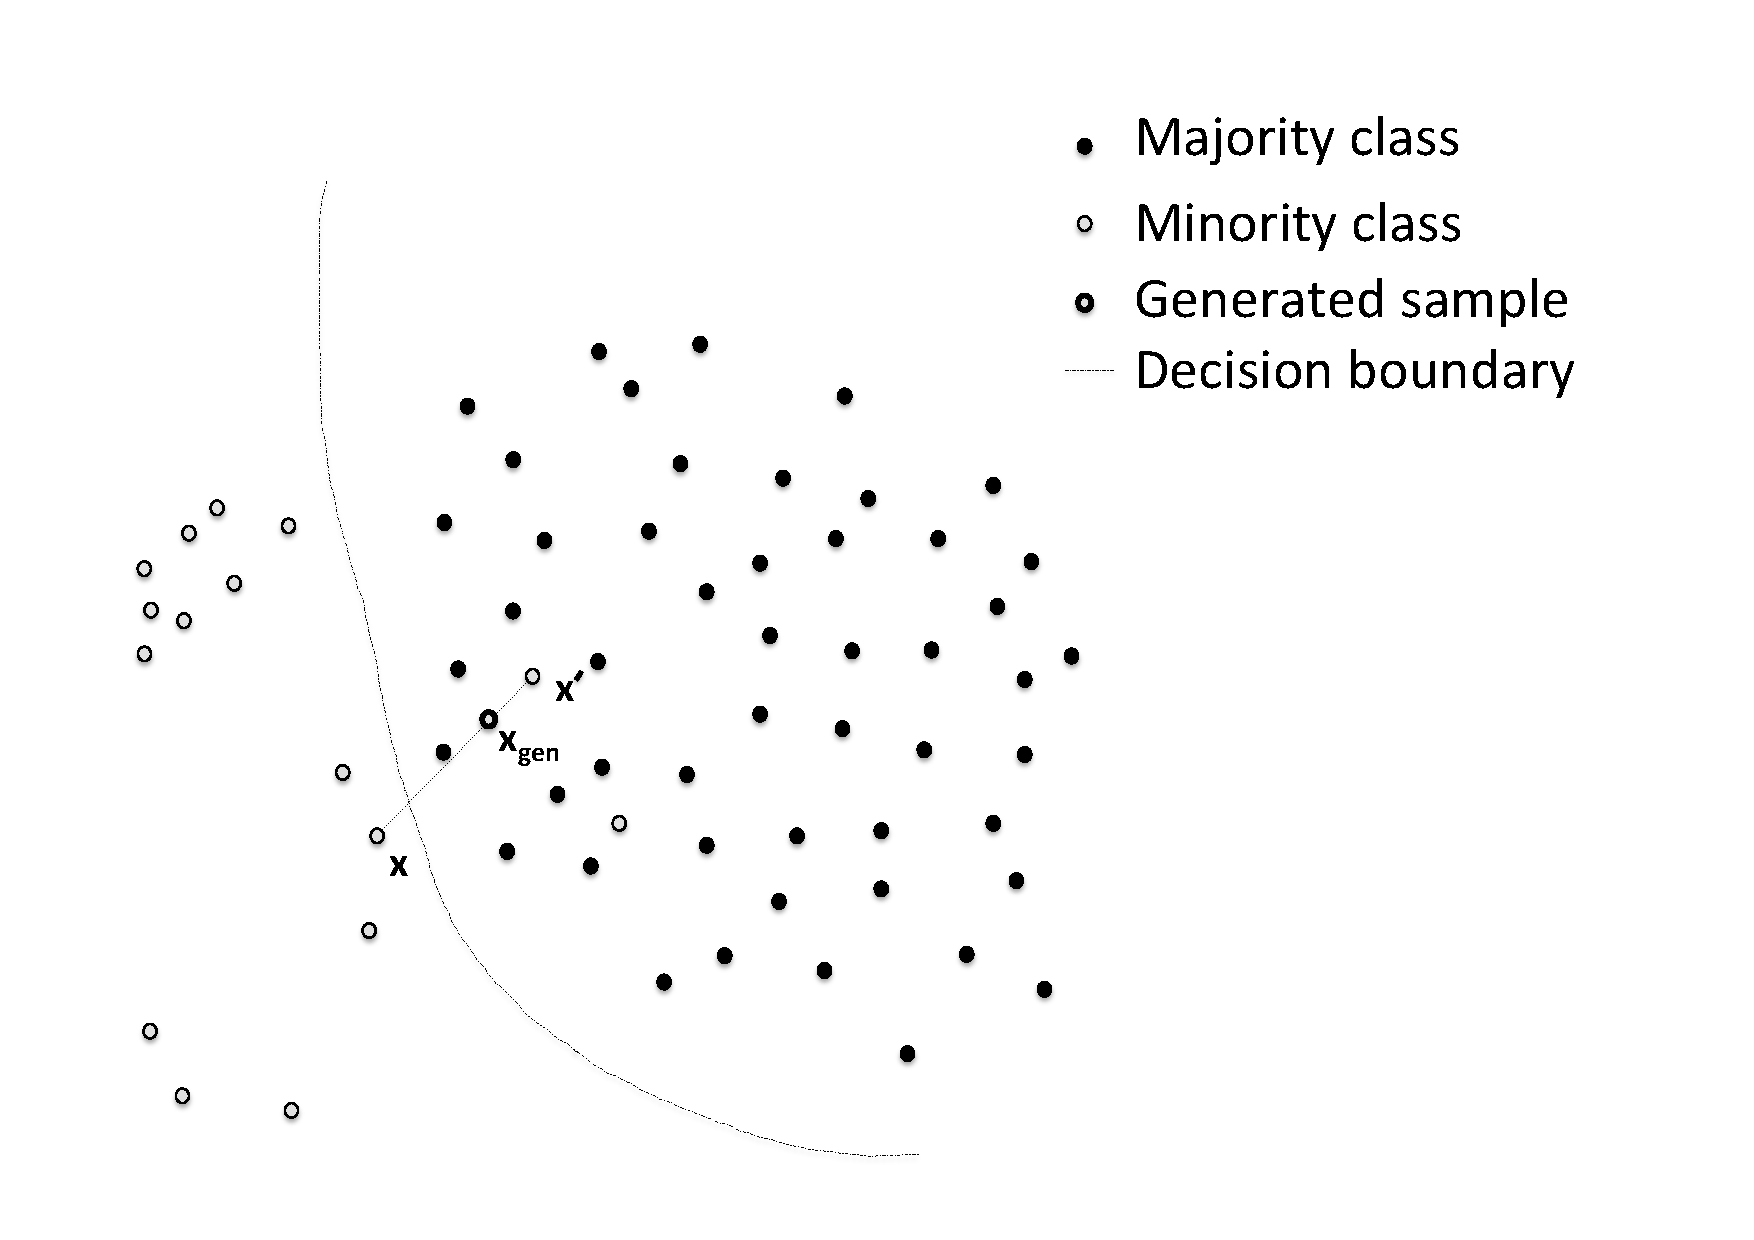
\includegraphics[width=12cm, keepaspectratio]{../resources/fig1}
	\captionbelow{An instance near the decision boundary and one of its 4-nearest neighbors are selected randomly. A noisy observation is generated.}
\end{figure}

2. \textit{Generation of noisy examples due to the selection of an initial observation.}

In order to avoid the previous scenario \( k \) is set to a small value. This choice does not eliminate the generation of noisy samples when \( x \) itself is a noisy instance as can be seen in Fig. 2.

\begin{figure}[H]
	\centering
	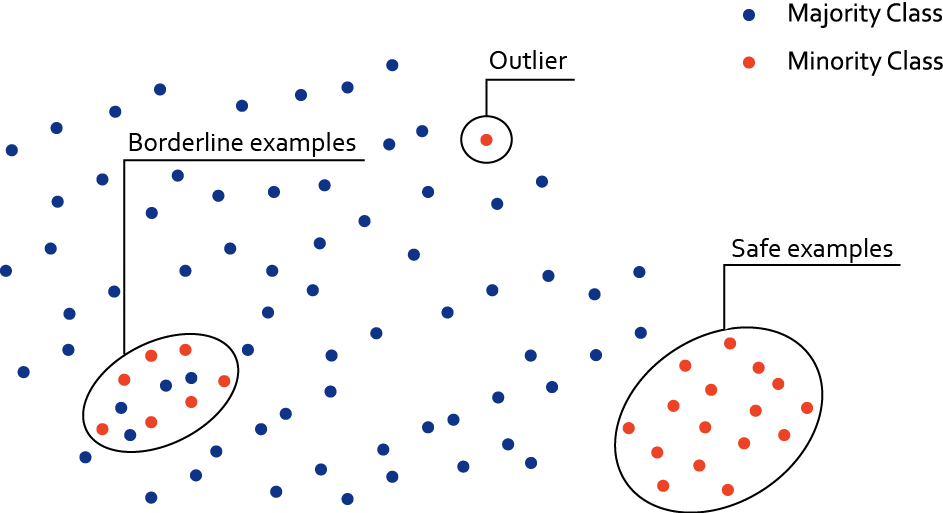
\includegraphics[width=12cm, keepaspectratio]{../resources/fig2}
	\captionbelow{A 2-nearest neighbor does not avoid the generation of noise when noisy samples are initially selected.}
\end{figure}

3. \textit{Generation of nearly duplicated instances.}

Minority and majority regions can be organized in different clusters, having complex decision boundaries.  In this case, being conservative in the selection of \( k \) may be a valid strategy since a small value of it can minimize the probability of generating noisy instances. On the other hand, it may increase the probability of generating synthetic instances in dense minority class areas as is shown in Fig 3, where \(x\) and \(x'\) belong in to the same cluster. These artificial samples are less useful because they do not add new information to the data set and are conducive to overfitting. Consequently, it is desirable to expand the data generation process in areas where minority examples are absent.

\begin{figure}[H]
	\centering
	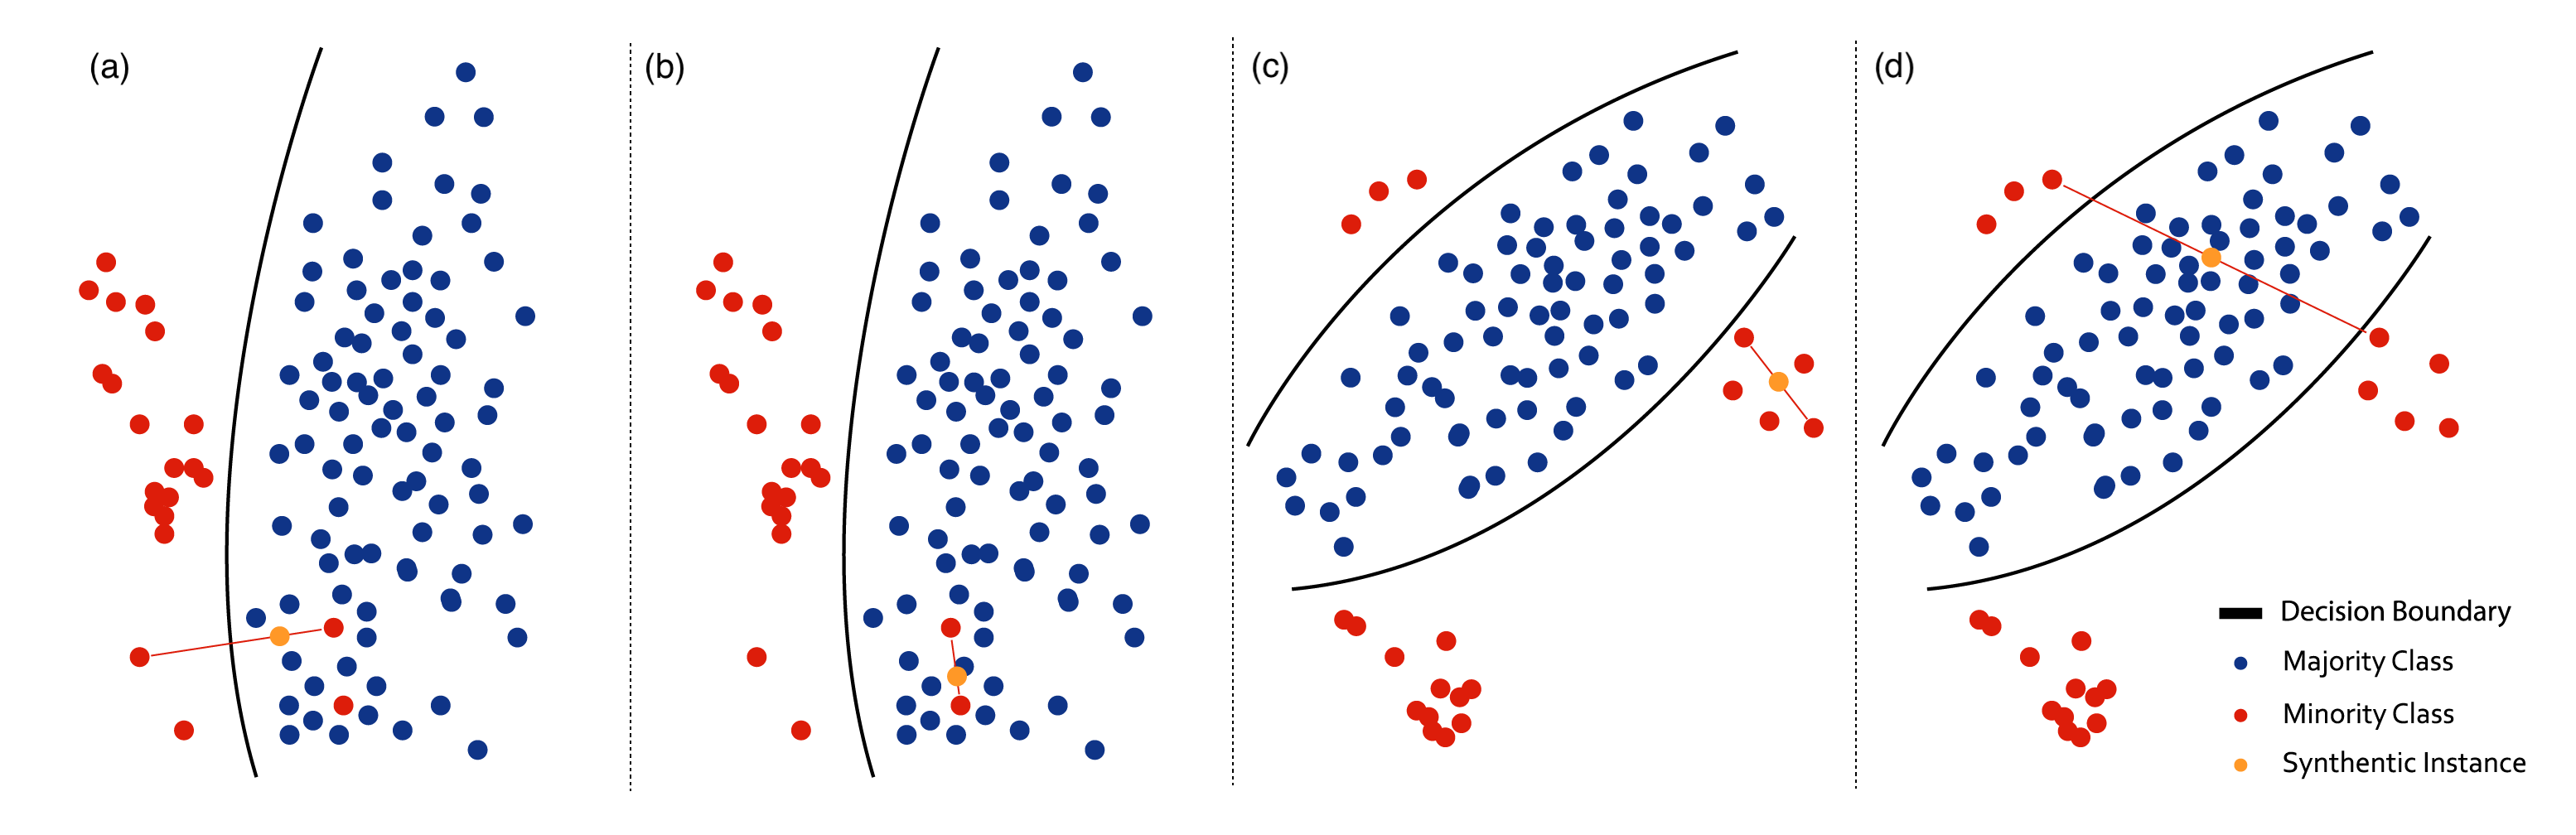
\includegraphics[width=12cm, keepaspectratio]{../resources/fig3}
	\captionbelow{An instance belonging to a minority class cluster and one of its 5-nearest neighbors are selected. An observation belonging to the same cluster is generated.}
	\end{figure}

4. \textit{Generation of noisy instances due to the use of observations from two different minority class clusters.}

Increasing \( k \)  in order to avoid the previous scenario,  may result to a selected \( x' \) such that \( x \) and \( x' \) belong to different clusters. This in turn may lead to the generation of a new instance within the majority region as it is exemplified in Fig. 4. 

\begin{figure}[H]
	\centering
	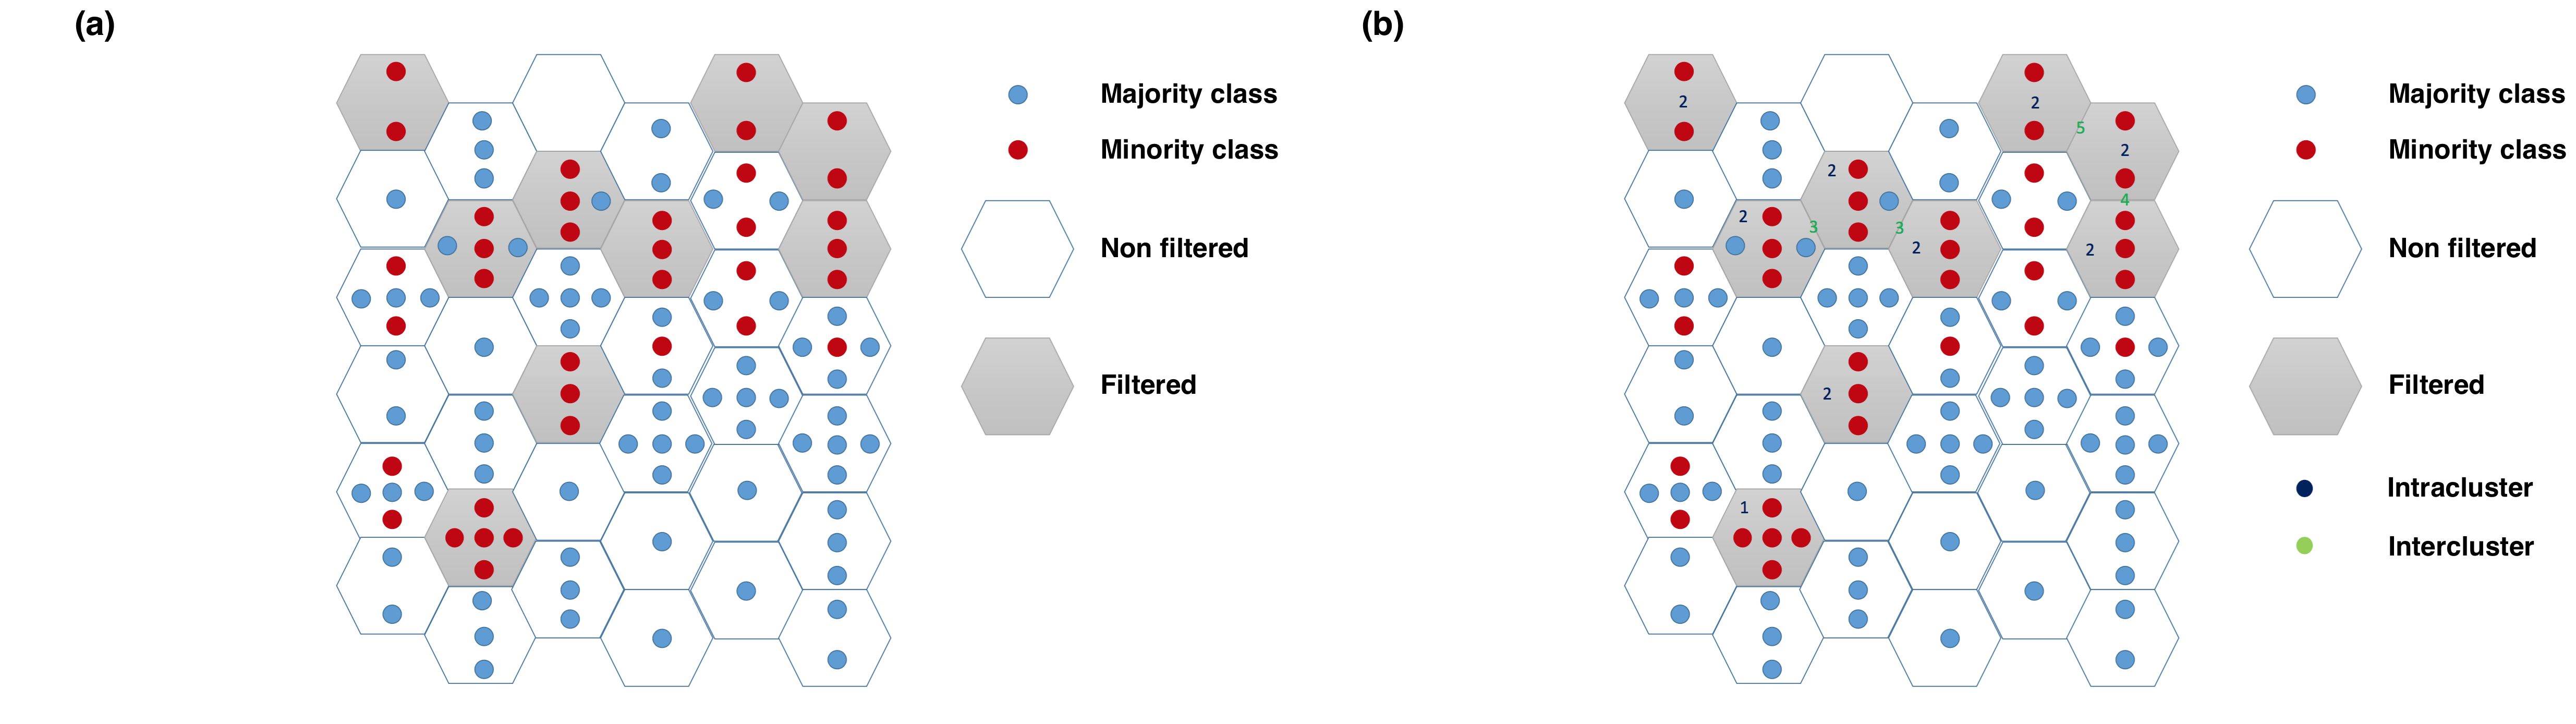
\includegraphics[width=12cm, keepaspectratio]{../resources/fig4}
	\captionbelow{An attempt to generate inter-cluster instances by increasing the number of k-nearest neighbors of the selected instances. One of the generated instances penetrates in the majority class area.}
\end{figure}

\section{The proposed method}

In the previous section some insufficiencies of the SMOTE data generation mechanism in various scenarios were described. Some of these insufficiencies apply also to other SMOTE-based oversamplers. We propose a novel data generation procedure, G-SMOTE, which is an extension of the SMOTE algorithm and has three main objectives:

1. \textit{To define a safe area around each selected minority class instance such that the generated artificial minority instances inside this area are not noisy.}

2. \textit{To increase the variety of generated samples by expanding the minority class area.}

3. \textit{To parametrize the above characteristics based on a small number of transformations with a geometrical interpretation.}

G-SMOTE can be considered as a drop-in replacement for SMOTE in the sense that any method relying on the SMOTE data generation mechanism can replace it with the one proposed by G-SMOTE without any further modifications. As it was mentioned on the previous sections, in this paper we aim to a direct comparison of the two data generation mechanisms, with the effect of the above replacement being an investigation of future work.

The complete algorithm in pseudo-code is presented in the following figure:

\begin{algorithm}
	
	\BlankLine
	
	\DontPrintSemicolon
	\KwIn{\( S_{maj}, S_{min}, N, k, \alpha_{sel}, \alpha_{trunc}, \alpha_{def} \) }
	\KwOut{\( S_{gen}  \)}
	
	\BlankLine
	\BlankLine
	
	\SetKwFunction{Surface}{Surface}
	\SetKwProg{Pn}{Function}{:}{}
	\Pn{\Surface{\( \alpha_{sel} \), \( \textbf{x}_{center} \), \( S_{maj} \), \( S_{min} \) }}{
		\If{\( \alpha_{sel} = minority \)}
		{
			\( \textbf{x}_{surface} \in S_{min, k}\)\;
		}
		\ElseIf {\( \alpha_{sel} = majority \)}
		{
			\( \textbf{x}_{surface} \in S_{maj, 1}\)\;
		}
		\ElseIf {\( \alpha_{sel} = combined \)}
		{
			\( \textbf{x}_{min} \in S_{min, k}\)\;
			\( \textbf{x}_{maj} \in S_{maj, 1}\)\;
			\( \textbf{x}_{surface} \leftarrow \displaystyle argmin_{\textbf{x}_{min}, \textbf{x}_{maj}} \Big( \| \textbf{x}_{center} - \textbf{x}_{min} \|, \| \textbf{x}_{center} - \textbf{x}_{maj} \| \Big) \) \;
		}
		\KwRet\  \( \textbf{x}_{surface} \) \;
	}
	
	\BlankLine
	\BlankLine
	
	\SetKwFunction{Vectors}{Vectors}
	\SetKwProg{Pn}{Function}{:}{}
	\Pn{\Vectors{\( \textbf{x}_{center} \), \( \textbf{x}_{surface} \)}}{
		\( \textbf{e}_{\scriptscriptstyle//} \leftarrow \frac{\textbf{x}_{surface} - \textbf{x}_{center}}{ \| \textbf{x}_{surface} - \textbf{x}_{center} \|}  \) \;
		\( \textbf{x}_{\scriptscriptstyle//} \leftarrow ( \textbf{x}_{gen} \cdot \textbf{e}_{\scriptscriptstyle//} )  \ \textbf{e}_{\scriptscriptstyle//}  \) \;
		\( \textbf{x}_{\bot} \leftarrow \textbf{x}_{gen} - \textbf{x}_{\scriptscriptstyle//} \) \;
		
		\KwRet\  \( (\textbf{x}_{\scriptscriptstyle//}, \textbf{x}_{\bot}) \) \;
	}
	
	\BlankLine
	\BlankLine
	
	\SetKwFunction{Hyperball}{Hyperball}
	\SetKwProg{Pn}{Function}{:}{}
	\Pn{\Hyperball{}}{
		\( v_{i} \sim N(0, 1) \) \;
		\( r \sim U(0, 1) \) \;
		\( \textbf{x}_{gen} \leftarrow r^{1 / p} \frac{ (v_{1}, \cdots, v_{p}) }{\| (v_{1}, \cdots, v_{p}) \| }  \) \;
		\KwRet\  \( \textbf{x}_{gen} \) \;
	}
	
	\BlankLine
	\BlankLine
	
	\SetKwFunction{Truncate}{Truncate}
	\SetKwProg{Pn}{Function}{:}{}
	\Pn{\Truncate{\( \alpha_{trunc}, \textbf{x}_{gen}, \textbf{x}_{center}, \textbf{x}_{surface} \)}}{
		\If{ \( |\alpha_{trunc} - x_{\scriptscriptstyle//}| > 1 \) }
		{
			\( \textbf{x}_{gen} \leftarrow \textbf{x}_{gen} - 2 \textbf{x}_{\scriptscriptstyle//} \) \;
		}
		\KwRet\  \( \textbf{x}_{gen} \) \;
	}
	
	\BlankLine
	\BlankLine
	
	\SetKwFunction{Deform}{Deform}
	\SetKwProg{Pn}{Function}{:}{}
	\Pn{\Deform{\( \alpha_{dist}, \textbf{x}_{gen}, \textbf{x}_{center}, \textbf{x}_{surface} \) }} {
		\KwRet\  \(  \textbf{x}_{gen} - \alpha_{def} \ \textbf{x}_{\bot}  \) \;
	}
	
	\BlankLine
	\BlankLine
	
	\SetKwFunction{Translate}{Translate}
	\SetKwProg{Pn}{Function}{:}{}
	\Pn{\Translate{\(  \textbf{x}_{gen}, \textbf{x}_{center}, R \) }} {
		\KwRet\  \(  \textbf{x}_{center} +  R \ \textbf{x}_{gen} \) \;
	}
	
	\BlankLine
	\BlankLine

	\Begin{
		\nl\( S_{gen} = \emptyset \)\;
		\nl\While{\( \vert S_{gen} \vert < N \) }{
			\nl\( \textbf{x}_{center} \in \ S_{min} \) \;
			\nl\( \textbf{x}_{surface} \leftarrow \) \Surface{\( \alpha_{sel} \), \( \textbf{x}_{center} \), \( S_{maj} \), \( S_{min} \) }  \;
			\nl\( (\textbf{x}_{\scriptscriptstyle//}, \textbf{x}_{\bot}) \leftarrow \) \Vectors{ \( \textbf{x}_{center} \), \( \textbf{x}_{surface} \) } \;
			\nl\( \textbf{x}_{gen} \leftarrow \) \Hyperball{}  \;
			\nl\( \textbf{x}_{gen} \leftarrow \)  \Truncate{\( \alpha_{trunc}, \textbf{x}_{gen}, \textbf{x}_{center}, \textbf{x}_{surface} \) } \;
			\nl\( \textbf{x}_{gen} \leftarrow \)  \Deform{ \(  \alpha_{dist}, \textbf{x}_{gen}, \textbf{x}_{center}, \textbf{x}_{surface} \) } \;
			\nl\( \textbf{x}_{gen} \leftarrow \)  \Translate{ \(  \textbf{x}_{gen}, \textbf{x}_{center}, \| \textbf{x}_{center} - \textbf{x}_{surface} \| \) } \;
			\nl\( S_{gen} \leftarrow S_{gen} \cup \{ \textbf{x}_{gen} \} \)\;
		}
	}

	\caption{G-SMOTE}\label{gsmote}
	
\end{algorithm}

\subsection{G-SMOTE algorithm}

The inputs of the G-SMOTE algorithm are the following: 

\begin{itemize}

\renewcommand\labelitemi{--}

\item The sets \( S_{maj} \),  \( S_{min} \) of majority and minority class samples, respectively.

\item The total number \( N \) of synthetic samples to be generated.

\item The number \( k \) of nearest neighbors.

\item The neighbor selection strategy \( \alpha_{sel} \) with \( \alpha_{sel} \in \Big\{ minority, majority, combined \Big\} \).

\item The truncation factor \( \alpha_{trunc} \) with \( -1 \leq \alpha_{trunc} \leq 1 \). 

\item The deformation factor \( \alpha_{def} \) with \( 0 \leq \alpha_{def} \leq 1 \).

\end{itemize}

The output of G-SMOTE is the set \( S_{gen} \) of generated synthetic examples.

The algorithmic procedure is the following:

\begin{itemize}
	
\renewcommand\labelitemi{--}

 \item The \( S_{min} \) elements are shuffled and an empty set \( S_{gen} \) is initialized. 
 
 \item The following loop is repeated until \( N \) minority instances are selected, each multiple times if necessary, in the order that appear in \( S_{min} \):
 
 	\begin{itemize}
 		
 		 \item Let \( \textbf{x}_{center} \in \ S_{min} \) the selected minority class instance of \( p \) components.
 		 
 		 \item A surface vector is defined from the relation \( \textbf{x}_{surface} \leftarrow \) \Surface{\( \alpha_{sel} \), \( \textbf{x}_{center} \), \( S_{maj} \), \( S_{min} \) } .
 		 
 		 \item A set of direction vectors \( (\textbf{x}_{\scriptscriptstyle//}, \textbf{x}_{\bot}) \leftarrow \) \Vectors{ \( \textbf{x}_{center} \), \( \textbf{x}_{surface} \) }  is extracted.
 		 
 		 \item A synthetic sample \( \textbf{x}_{gen} \leftarrow \) \Hyperball{} is generated.
 		 
 		 \item The transformation functions  \texttt{Truncate}, \texttt{Deform} and \texttt{Translate} are applied to \( \textbf{x}_{gen} \).
 		 
 		 \item \( \textbf{x}_{gen} \) is added to \( S_{gen} \).
 		
 	\end{itemize}

\end{itemize}

\subsection{Functions}

The above algorithmic procedure relies on the following definitions of functions:

\begin{itemize}
	
	\renewcommand\labelitemi{--}
	
	\item Function \texttt{Surface}:
	
		The sets  \( S_{min, k} \) and \( S_{maj, 1} \) are the sets of \( k \) and \( k = 1 \) nearest neighbors of \( \textbf{x}_{center} \) from \( S_{min} \) and \( S_{maj} \), respectively.
	
		If \( \alpha_{sel} = minority \) then an element \( \textbf{x}_{surface} \in S_{min, k}\) is randomly selected.
			
		If \( \alpha_{sel} = majority \) then an element \( \textbf{x}_{surface} \in S_{maj, 1}\) is randomly selected.
			
		If \( \alpha_{sel} = combined \) then \( S_{min, k} \) and \( S_{maj, 1} \) are defined as above and the elements \( \textbf{x}_{min} \in S_{min, k}\) and  \( \textbf{x}_{maj} \in S_{maj, 1}\) are randomly selected. Finally the element \( \textbf{x}_{surface} \) is defined as either \( \textbf{x}_{min} \) or \( \textbf{x}_{maj} \) by selecting the one with smallest distace from \( \textbf{x}_{center} \).
			
	
	\item Function \texttt{Hyperball}:
		
		A vector \( \textbf{v}_{normal} \leftarrow (v_{1}, \cdots, v_{p}) \) is generated of \( p \) random numbers from the normal distribution \( N(0, 1) \). The unit vector \( \textbf{e}_{sphere} \leftarrow \frac{\textbf{v}_{normal}}{ \|\textbf{v}_{normal} \|} \inlineeqnum\label{eqn:sphere} \) and the vector \( \textbf{x}_{gen} \leftarrow r^{1 / p} \textbf{e}_{sphere} \inlineeqnum\label{eqn:ball} \) are calculated where \( r \) is a random number from the uniform distribution \( U(0, 1) \).
			
	\item Function \texttt{Vectors}:
	
		The unit vector \( \textbf{e}_{\scriptscriptstyle//} \leftarrow \frac{\textbf{x}_{surface} - \textbf{x}_{center}}{ \|\textbf{x}_{surface} - \textbf{x}_{center} \|} \inlineeqnum\label{eqn:unit} \) and the projection  \( x_{\scriptscriptstyle//} = \textbf{x}_{gen} \cdot \textbf{e}_{\scriptscriptstyle//} \)  are defined. Using this projection, the vectors \( \textbf{x}_{\scriptscriptstyle//} \leftarrow x_{\scriptscriptstyle//} \textbf{e}_{\scriptscriptstyle//}  \inlineeqnum\label{eqn:parallel} \) and \( \textbf{x}_{\bot} \leftarrow \textbf{x}_{gen} - \textbf{x}_{\scriptscriptstyle//} \) are also defined.
	 		
	 \item Function \texttt{Truncate}:
	 
	 	If the relation \( |\alpha_{trunc} - x_{\scriptscriptstyle//}| > 1 \inlineeqnum\label{eqn:condition} \) holds then the transformation \( \textbf{x}_{gen} \leftarrow \textbf{x}_{gen} - 2 \textbf{x}_{\scriptscriptstyle//} \inlineeqnum\label{eqn:truncate} \) is applied.
	
	\item Function \texttt{Deform}: 
			
		The transformation \( \textbf{x}_{gen} \leftarrow \textbf{x}_{gen} - \alpha_{def} \  \textbf{x}_{\bot} \inlineeqnum\label{eqn:deform} \) is applied.
			
	\item Function \texttt{Translate}:
	
		The transformation \( \textbf{x}_{center} +  R \ \textbf{x}_{gen} \inlineeqnum\label{eqn:translate} \) is applied.
	
\end{itemize}

\subsection{Justification of the G-SMOTE algorithm}

As explained above, SMOTE compared to Random Oversampling, improves the diversity of generated samples by linearly interpolating generated samples between two minority class instances. However on high-dimensional data SMOTE does not change the class-specific mean values while it decreases the data variability and it introduces correlation between samples \cite{Blagus2013}. Contrary to this, G-SMOTE extends the linear interpolation mechanism by introducing a geometric region where the data generation process occurs. At the most general choice of hyper-parameters, this geometric region of the input space is a truncated hyper-spheroid. The various steps of the G-SMOTE algorithm can be described in detail as follows:

\begin{enumerate}
	
	\item An empty set \( S_{gen} \) is initialized. 

	\item The \( S_{min} \) elements are shuffled and the process described below is repeated \( N \) times until \( N \) artificial points have been generated.
	
	\item A minority class instance \( \textbf{x}_{center} \) is selected as the center of a geometric region. The order of selection follows the order of dataset points after shuffling on the previous step. Therefore if \( N \) is greater than \( S_{min} \), then some of the minority class samples will be selected more than once.

	\item At first glance, this step generalizes the selection phase of the SMOTE algorithm. More specifically, it results to a randomly selected sample called \( \textbf{x}_{surface} \) which might belong to either the minority or majority class, depending on the values of \( \alpha_{sel} \), \(k\) and \( \textbf{x}_{center} \). However, we consider it as a part of the G-SMOTE data generation mechanism since it does not just filters the selected minority class instances based on heuristic rules similarly to SMOTE variations. Based on the neighbor selection strategy \( \alpha_{sel} \), we distinguish 3 different cases:
	
	\begin{enumerate}

	\item Case \( \alpha_{sel} = minority \):

	In this case the neighbor selection strategy is based only on the minority class and it is identical to the selection strategy of SMOTE. Initially the \( k \) nearest neighbors of \( \textbf{x}_{center} \) from the set \( S_{min} \) are identified and one of them, \( \textbf{x}_{surface} \), is randomly selected. Fig. 5 presents an example of a minority class instance selection among the \( k = 4 \ \) nearest neighbors of \( \textbf{x}_{center} \). The time complexity of this selection strategy depends on the choice of the algorithm and increases with the dimensionality of the input space as well as the value of the \( k \) parameter \cite{Vaidya1989}. Therefore for a wide set of realistic cases restricting the search of nearest neighbors to the minority class has a lower computational cost than including the majority class instances in the search space.

	\begin{figure}[H]
		\centering
		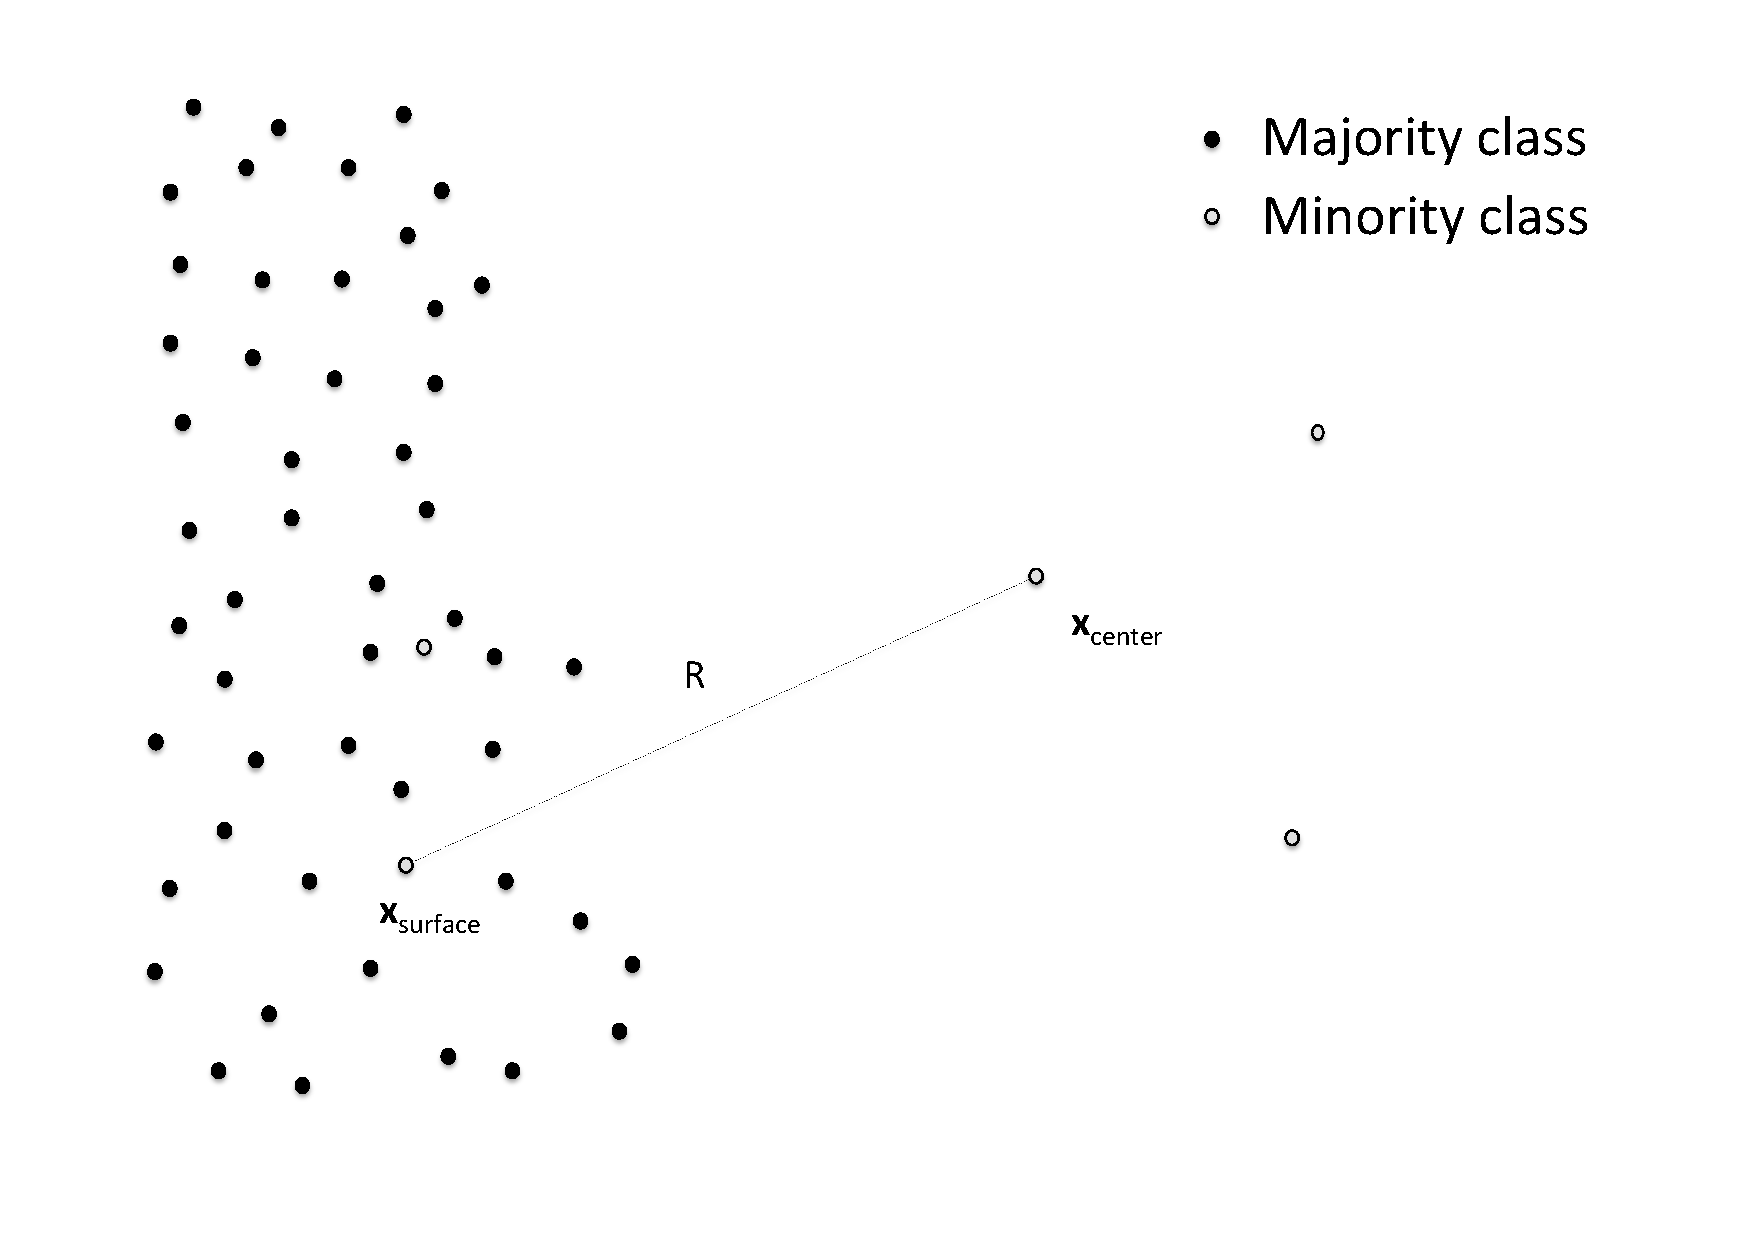
\includegraphics[width=12cm, keepaspectratio]{../resources/fig5}
		\captionbelow{An example of the minority selection strategy. A minority class instance is defined as the center of the hyper-spheroid and one of its \(k = 4\) minority class nearest neighbors is selected as the surface point. The radius \( R \) of the hyper-spheroid is defined to be equal to the distance of these minority instances.}
	\end{figure}

	\item Case \( \alpha_{sel} = majority \):

	As explained in section 3, one of the drawbacks of the minority selection strategy is that it may lead to the generation of data penetrating deeply in the majority class area. The majority selection strategy eliminates this scenario. More specifically, the nearest neighbor of \( \textbf{x}_{center} \) from the set \( S_{maj} \) is identified as \( \textbf{x}_{surface} \). The consequence of this selection is that when a random minority class point is generated inside a hypersphere of center \( \textbf{x}_{center} \) and radius \( R = \| \textbf{x}_{center} - \textbf{x}_{surface} \| \), it is ensured that its distance from \( \textbf{x}_{center} \) is not higher than the distance between \( \textbf{x}_{center} \) and any majority class instance. On the other hand, since any information about the minority class is discarded, this strategy might aggressively expand the minority class area, resulting effectively to noise generation. Fig. 6 presents an example of the nearest majority class instance selection among the majority class neighbors of \( \textbf{x}_{center} \). A disadvantage of the majority selection strategy is that the computational cost compared to the minority selection strategy may be higher, especially for datasets with high IR values.

	\begin{figure}[H]
		\centering
		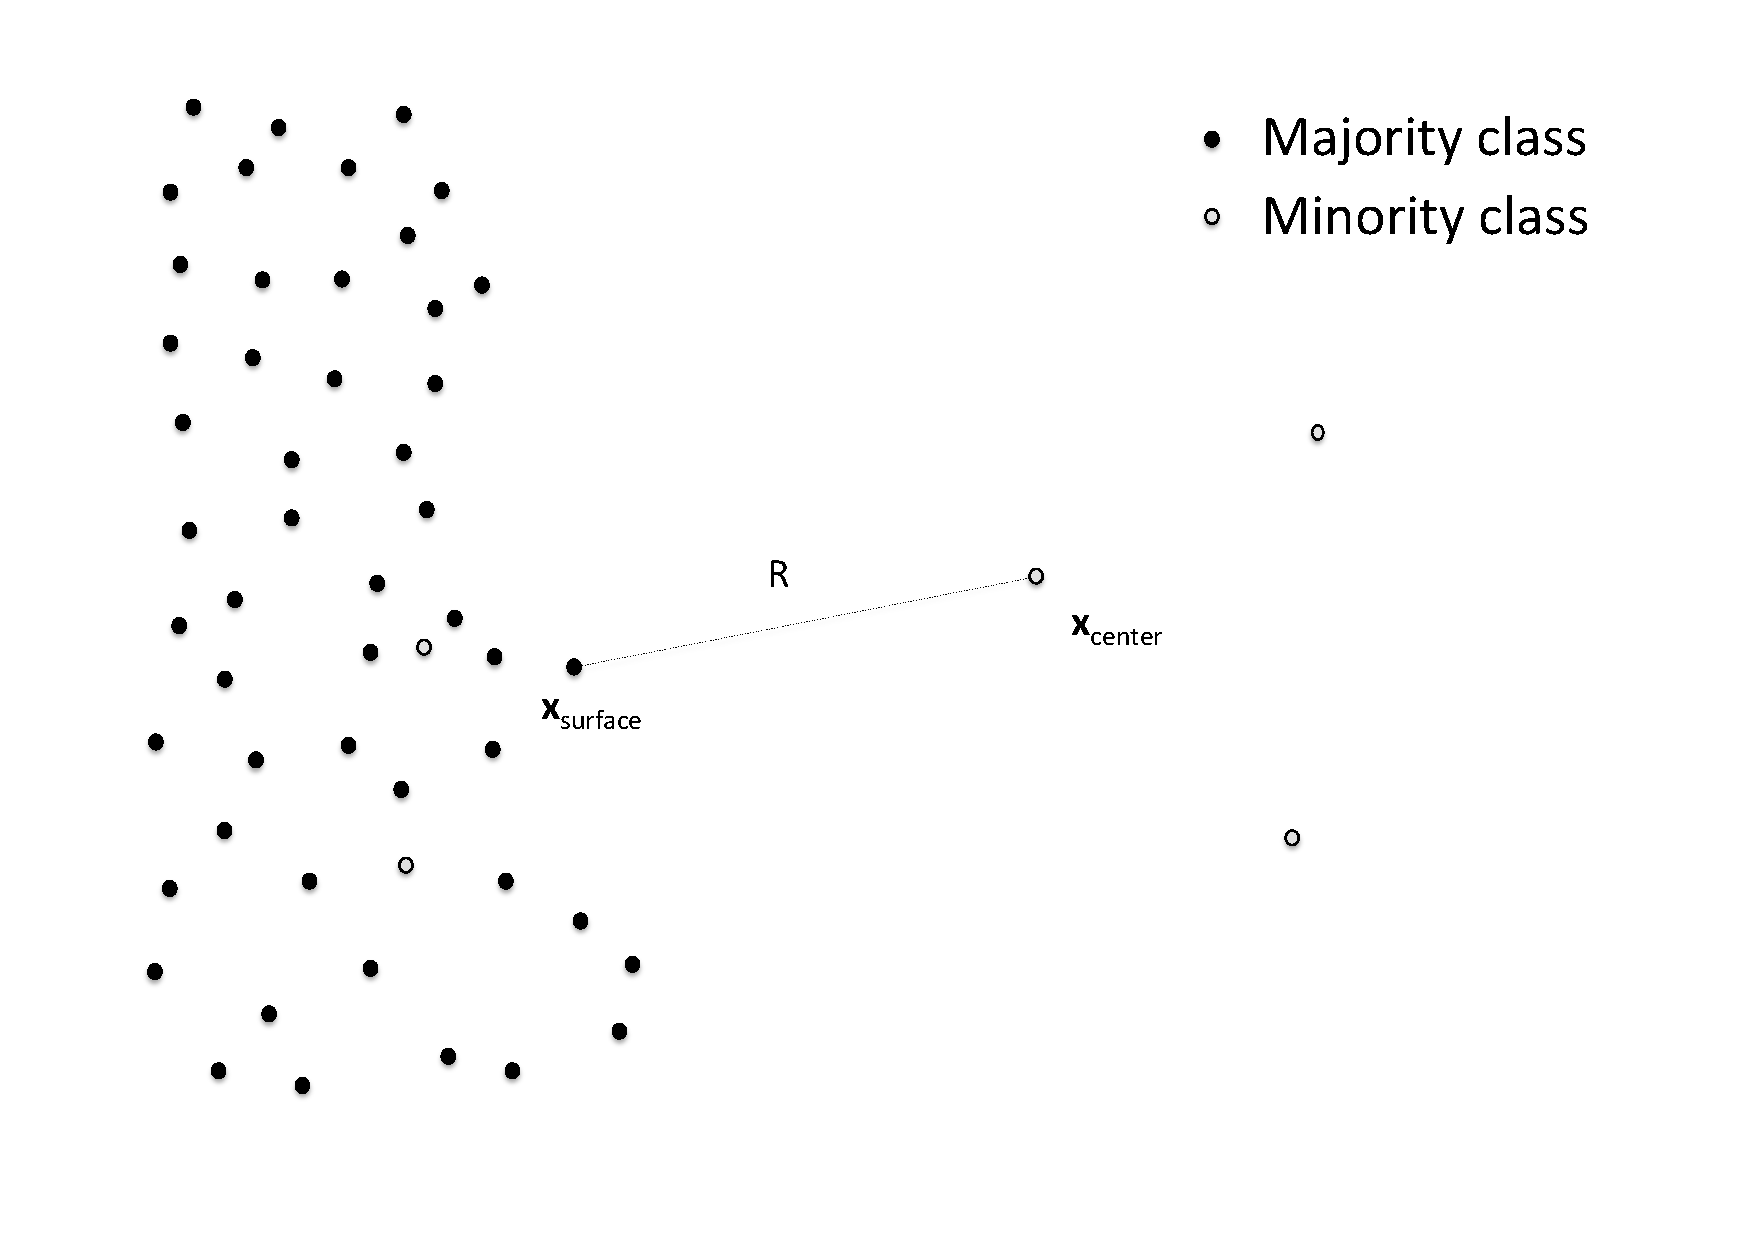
\includegraphics[width=12cm, keepaspectratio]{../resources/fig6}
		\captionbelow{An example of the majority selection strategy. A minority class instance is defined as the center of the hyper-spheroid and its closest majority class neighbor is selected as the surface point. The radius \( R \) of the hyper-spheroid is defined to be equal to the distance of these instances.}
	\end{figure}

	\item Case \( \alpha_{sel} = combined \):

	The combined selection strategy initially applies the minority and majority selection strategies, identifying \( \textbf{x}_{min} \) and \( \textbf{x}_{maj} \) as the selected minority and majority class instances, respectively. The surface point \( \textbf{x}_{surface} \) is defined to be either \( \textbf{x}_{min} \) or \( \textbf{x}_{maj} \), so that its distance from the center \( \textbf{x}_{center} \) is minimized. Fig. 7 and Fig. 8 present both of these scenarios i.e. when \( \textbf{x}_{surface} \) is identified either as a minority or majority class instance. Following the combined selection strategy, the expansion of the minority class area relative to the selected as a center minority class sample is restricted by the nearest majority class neighbor of the center, ensuring that the generation of noisy samples is avoided. Contrary to pure majority selection strategy, the expansion is not only safe but it is further restricted by the presence of minority class instances. The drawback of the combined, similarly to the majority selection strategy, is that it has a higher computational cost compared to the SMOTE/minority selection strategy.

	\begin{figure}[H]
		\centering
		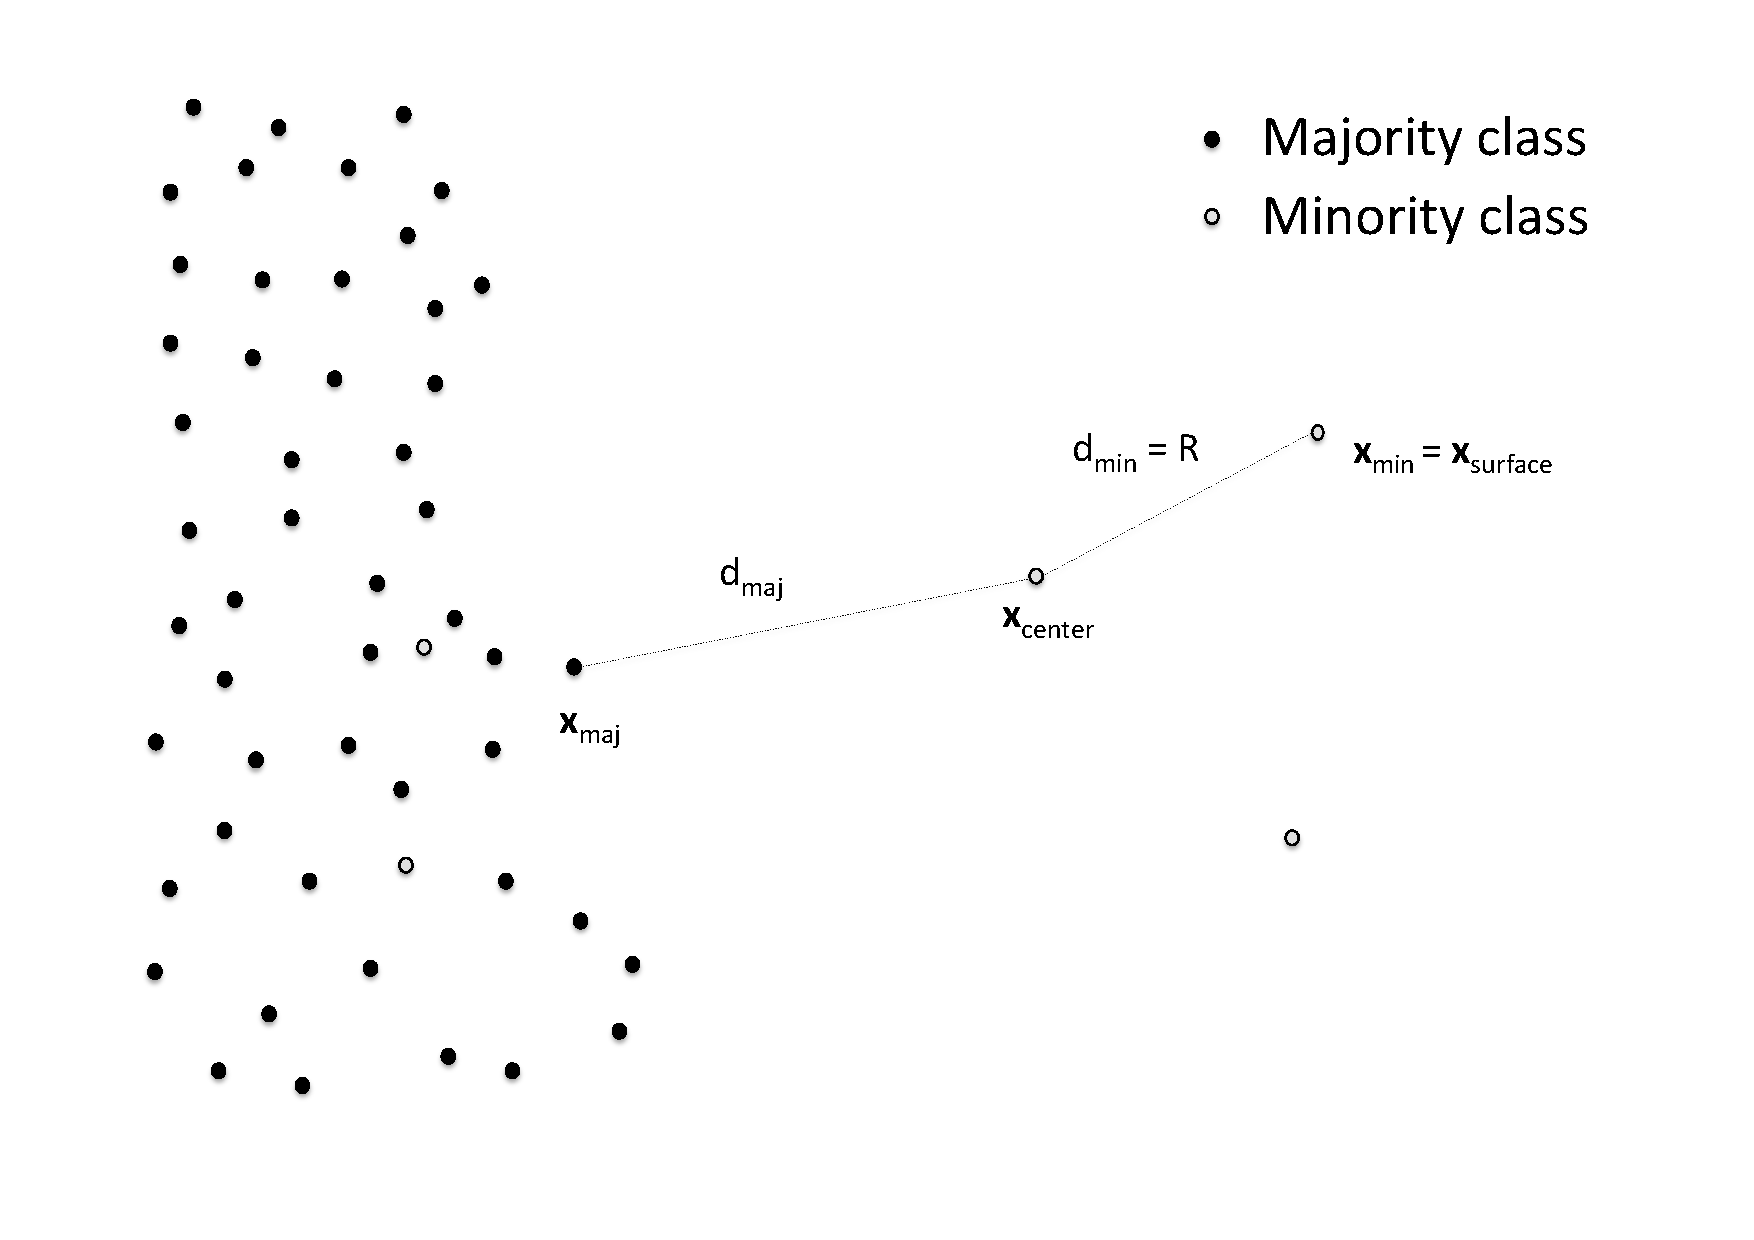
\includegraphics[width=12cm, keepaspectratio]{../resources/fig7}
		\captionbelow{A minority class sample is identified as the surface point since it is closer to the center than the nearest majority class instance.}
	\end{figure}

	\begin{figure}[H]
		\centering
		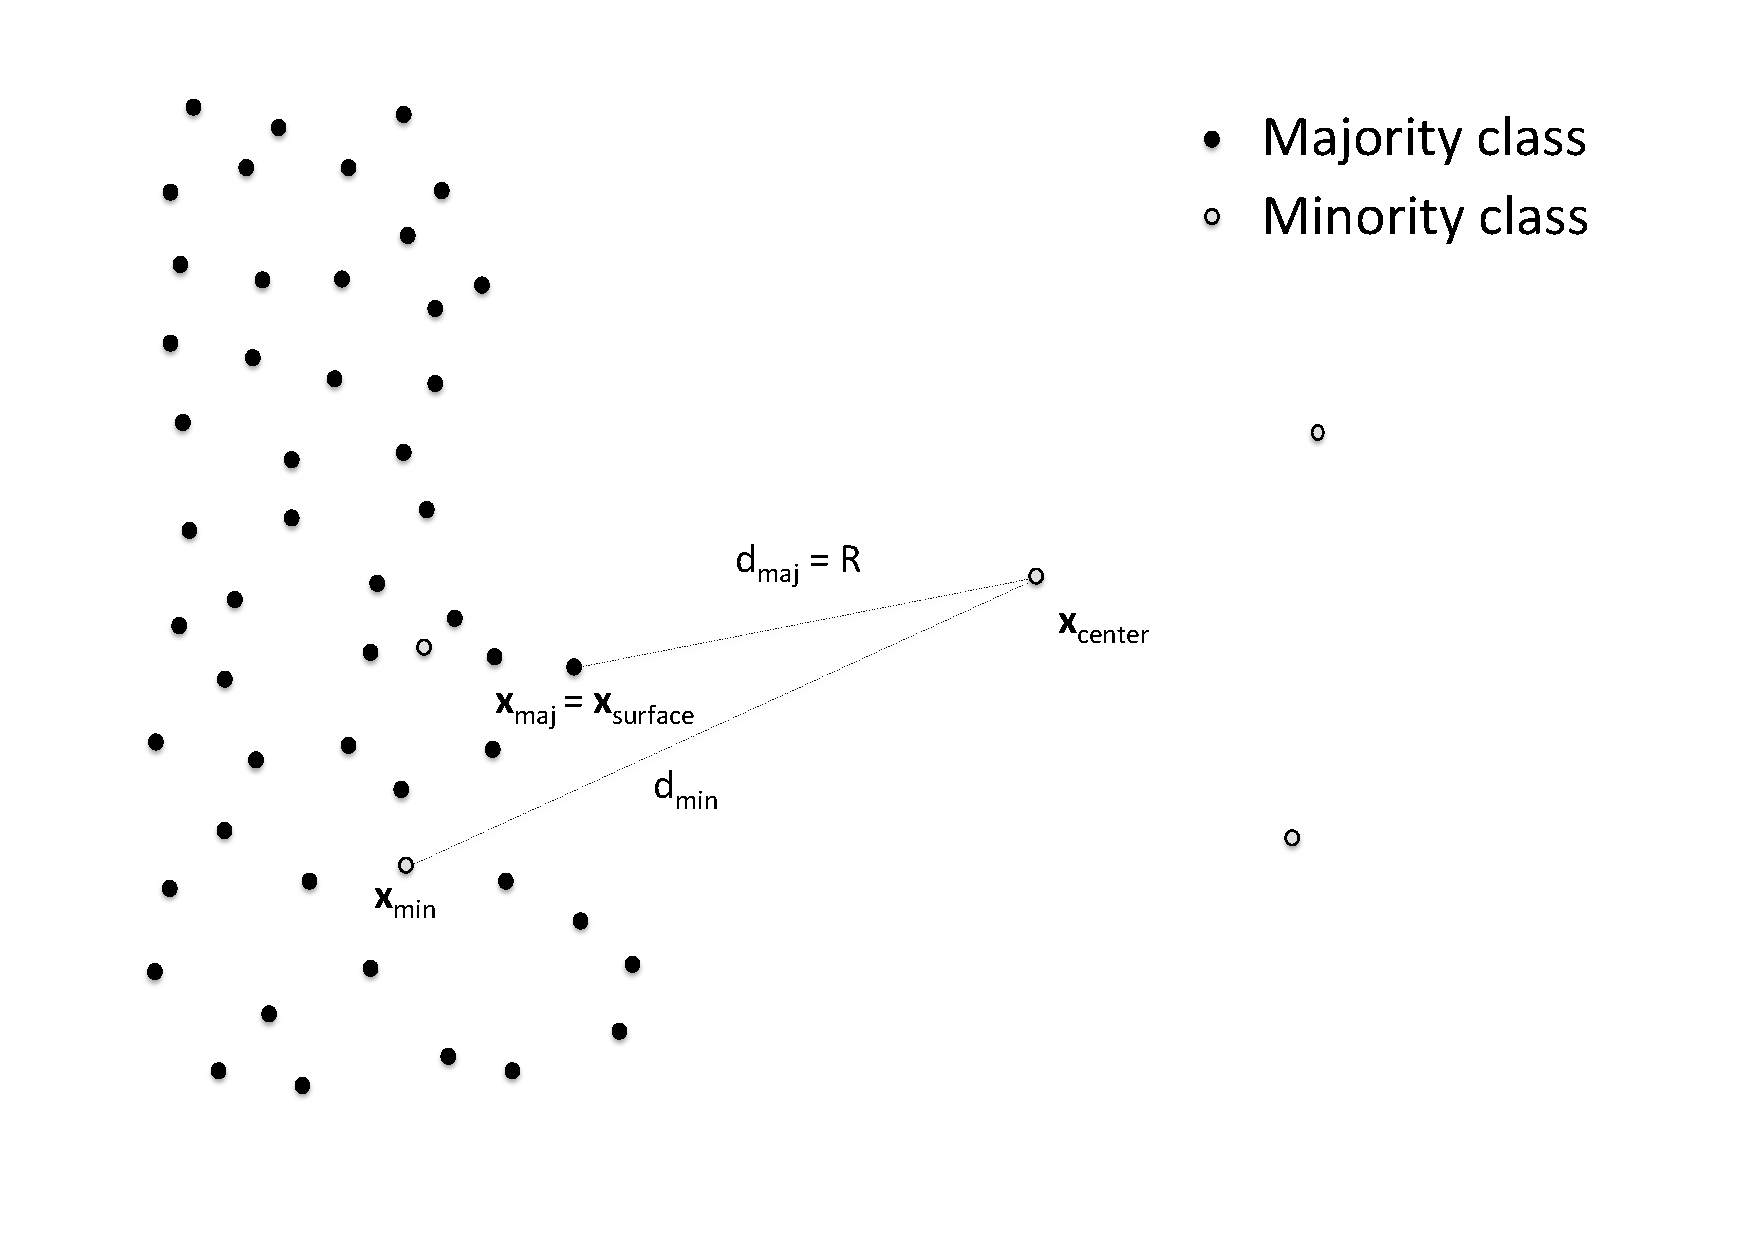
\includegraphics[width=12cm, keepaspectratio]{../resources/fig8}
		\captionbelow{The closest to the center majority class sample is identified as the surface point since it is closer to the center than the selected instance from the k nearest minority class neighbors of the center.}
	\end{figure}

	\end{enumerate}

	\item Two special directions in the input space are generated: \( \textbf{x}_{\scriptscriptstyle//} \) and \( \textbf{x}_{\bot} \). The first one represents the projection of \( \textbf{x}_{gen} \) to the unit vector \( \textbf{e}_{\scriptscriptstyle//} \) of equation \eqref{eqn:unit} that connects \( \textbf{x}_{center} \) to \( \textbf{x}_{surface} \), while the second is perpendicular to the same vector belonging also to the hyperplane defined by \( \textbf{x}_{gen} \) and \( \textbf{e}_{\scriptscriptstyle//} \).

	\item This step starts the data generation process. A random point \( \textbf{e}_{sphere} \) is generated on the surface of a unit hyper-sphere centered at the origin of the input space, using equation \eqref{eqn:sphere}. Applying equation \eqref{eqn:ball}, the point \( \textbf{e}_{sphere} \) is transformed to a random generated point \( \textbf{x}_{gen} \) inside the unit hyper-sphere. The final result of this process is a random generated point, uniformly distributed, within the unit hyper-sphere \cite{DasGupta2011}. Fig. 9 shows an example in two dimensions.

	\begin{figure}[H]
		\centering
		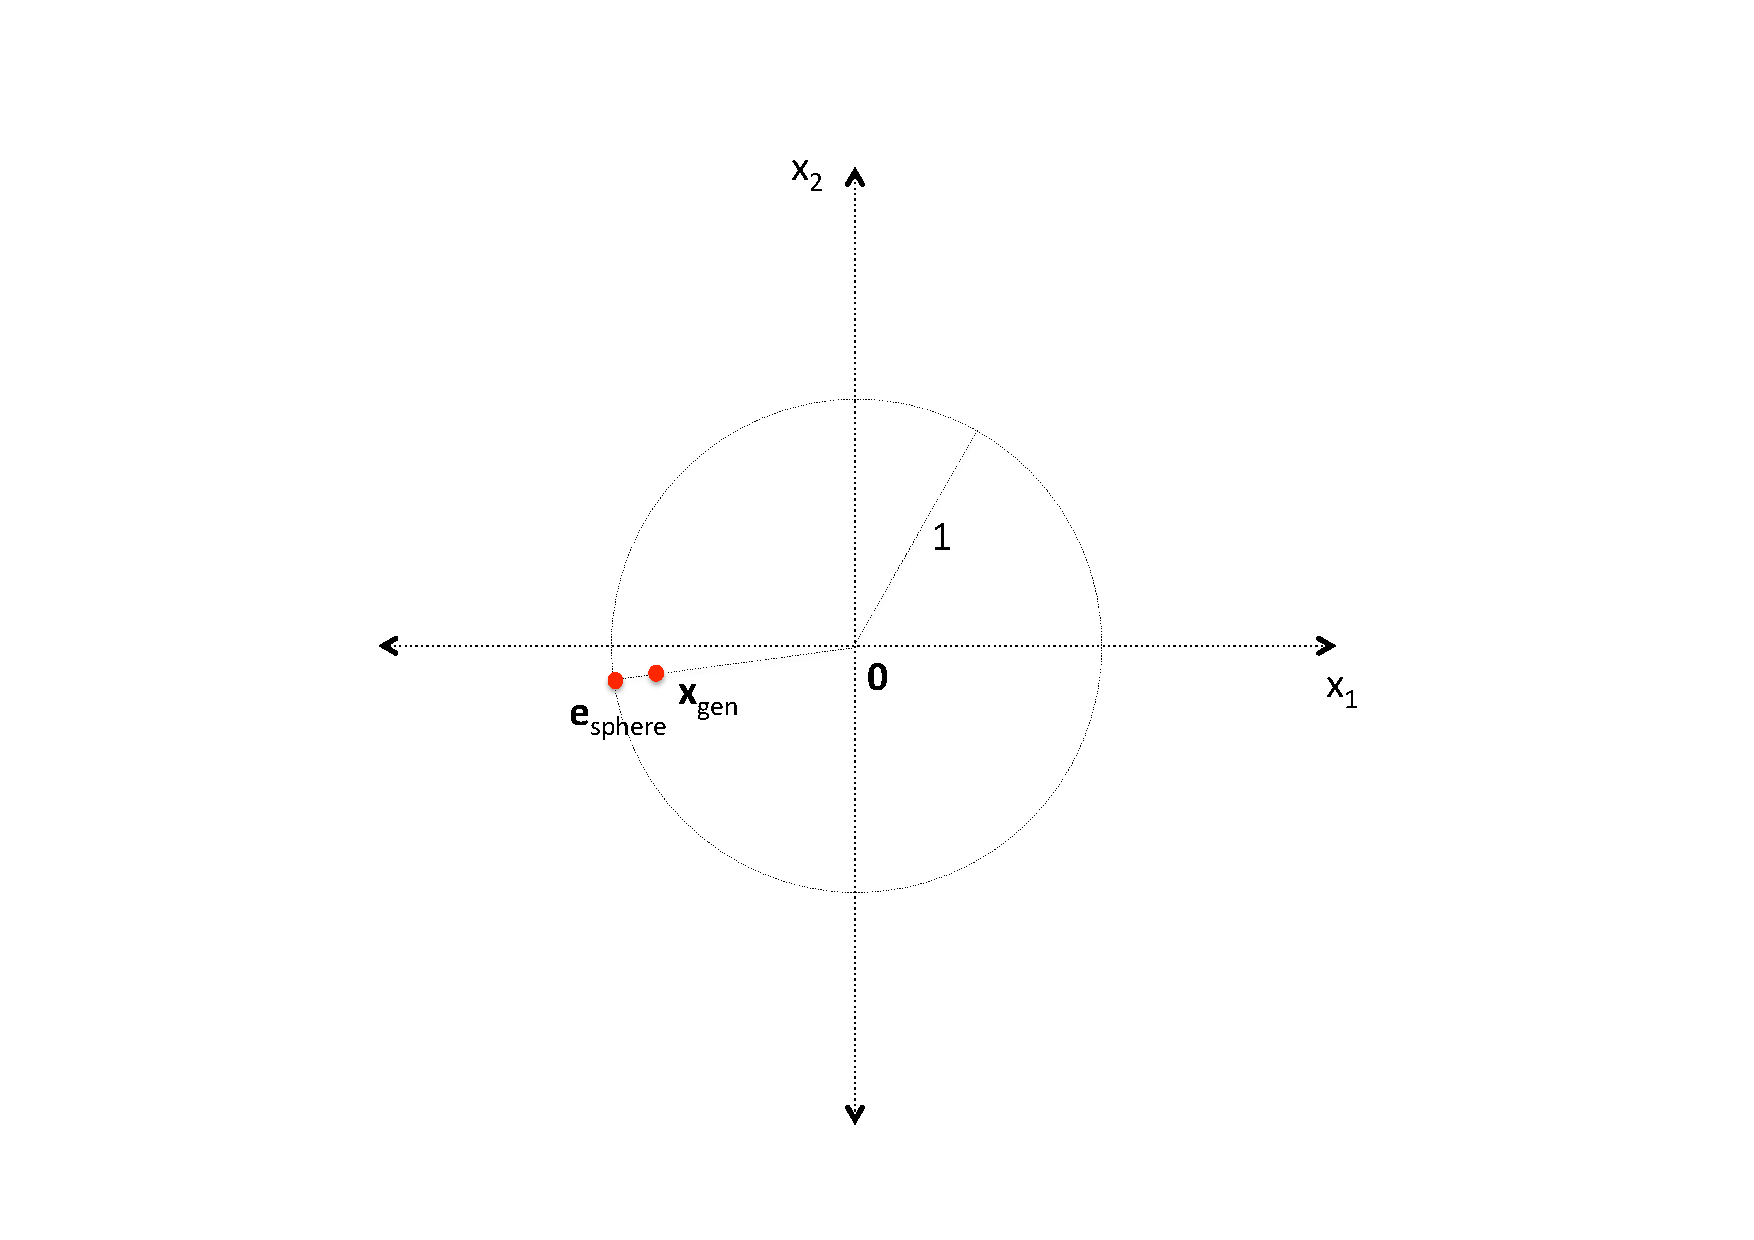
\includegraphics[width=12cm, keepaspectratio]{../resources/fig9}
		\captionbelow{A unit hyper-sphere centered at the origin of the input space. A point is randomly generated on the surface and moved to the interior of the unit hyper-sphere.}
	\end{figure}

	\item In this step a transformation is applied to the generated point \( \textbf{x}_{gen} \). As it was explained above, the center \( \textbf{x}_{center} \) and the selected surface point \( \textbf{x}_{surface} \) define a special direction in the input space which is represented by the unit vector \( \textbf{e}_{\scriptscriptstyle//} \) of equation \eqref{eqn:unit}. SMOTE mechanism, that always selects a minority class instance as a surface point, exploits this direction by generating synthetic samples at the line segment between \( \textbf{x}_{center} \) and \( \textbf{x}_{surface} \). G-SMOTE algorithm parametrizes a generalized version of the SMOTE mechanism. More specifically, the unit vector \( \textbf{e}_{\scriptscriptstyle//} \) defines a family of parallel hyper-planes which are perpendicular to it. We define a linear mapping between \( \alpha_{trunc} \) and the point determined by the intersection of each hyper-plane and the parallel to \( \textbf{e}_{\scriptscriptstyle//} \) diameter. Therefore each one of these hyper-planes corresponds to a particular value of \( \alpha_{trunc} \) and partitions the hyper-sphere interior in to two areas. Let \( P \) the hyper-plane that passes through the origin and \( P' \) the hyper-plane for a specific non-zero value of \( \alpha_{trunc} \). When \( a_{trunc} > 0 \), the area that does not include the \( \textbf{e}_{\scriptscriptstyle//} \) point is truncated from the interior of the hyper-sphere, in the sense that if the \( \textbf{x}_{gen} \) point belongs to it then it is mapped with respect to \( P \) to the symmetric point \( \textbf{x}_{gen} - 2 \textbf{x}_{\scriptscriptstyle//} \) of equation  \eqref{eqn:truncate}, where \( \textbf{x}_{\scriptscriptstyle//} \) is defined in equation \eqref{eqn:parallel}. Condition  \eqref{eqn:condition} checks if  the \( \textbf{x}_{gen} \) is in the truncated area. Fig. 10 shows an example of the above transformation. When \( \alpha_{trunc} < 0 \), the transformation is similarly defined but in this case the truncation occurs in the area that includes the \( \textbf{e}_{\scriptscriptstyle//} \) point. In both cases, the absolute value of the hyper-parameter \( \alpha_{trunc} \) controls the extent of the truncation. Fig. 11 presents the truncated hyper-sphere areas for various positive and negative values of \( \alpha_{trunc} \). A final observation is that the above transformation effectively corresponds to a modification of the initial uniform probability distribution in the hyper-sphere. The truncated area acquires a zero value for the p.d.f., while its \( P \)-symmetric mapped area doubles its initial p.d.f. value.

	\begin{figure}[H]
		\centering
		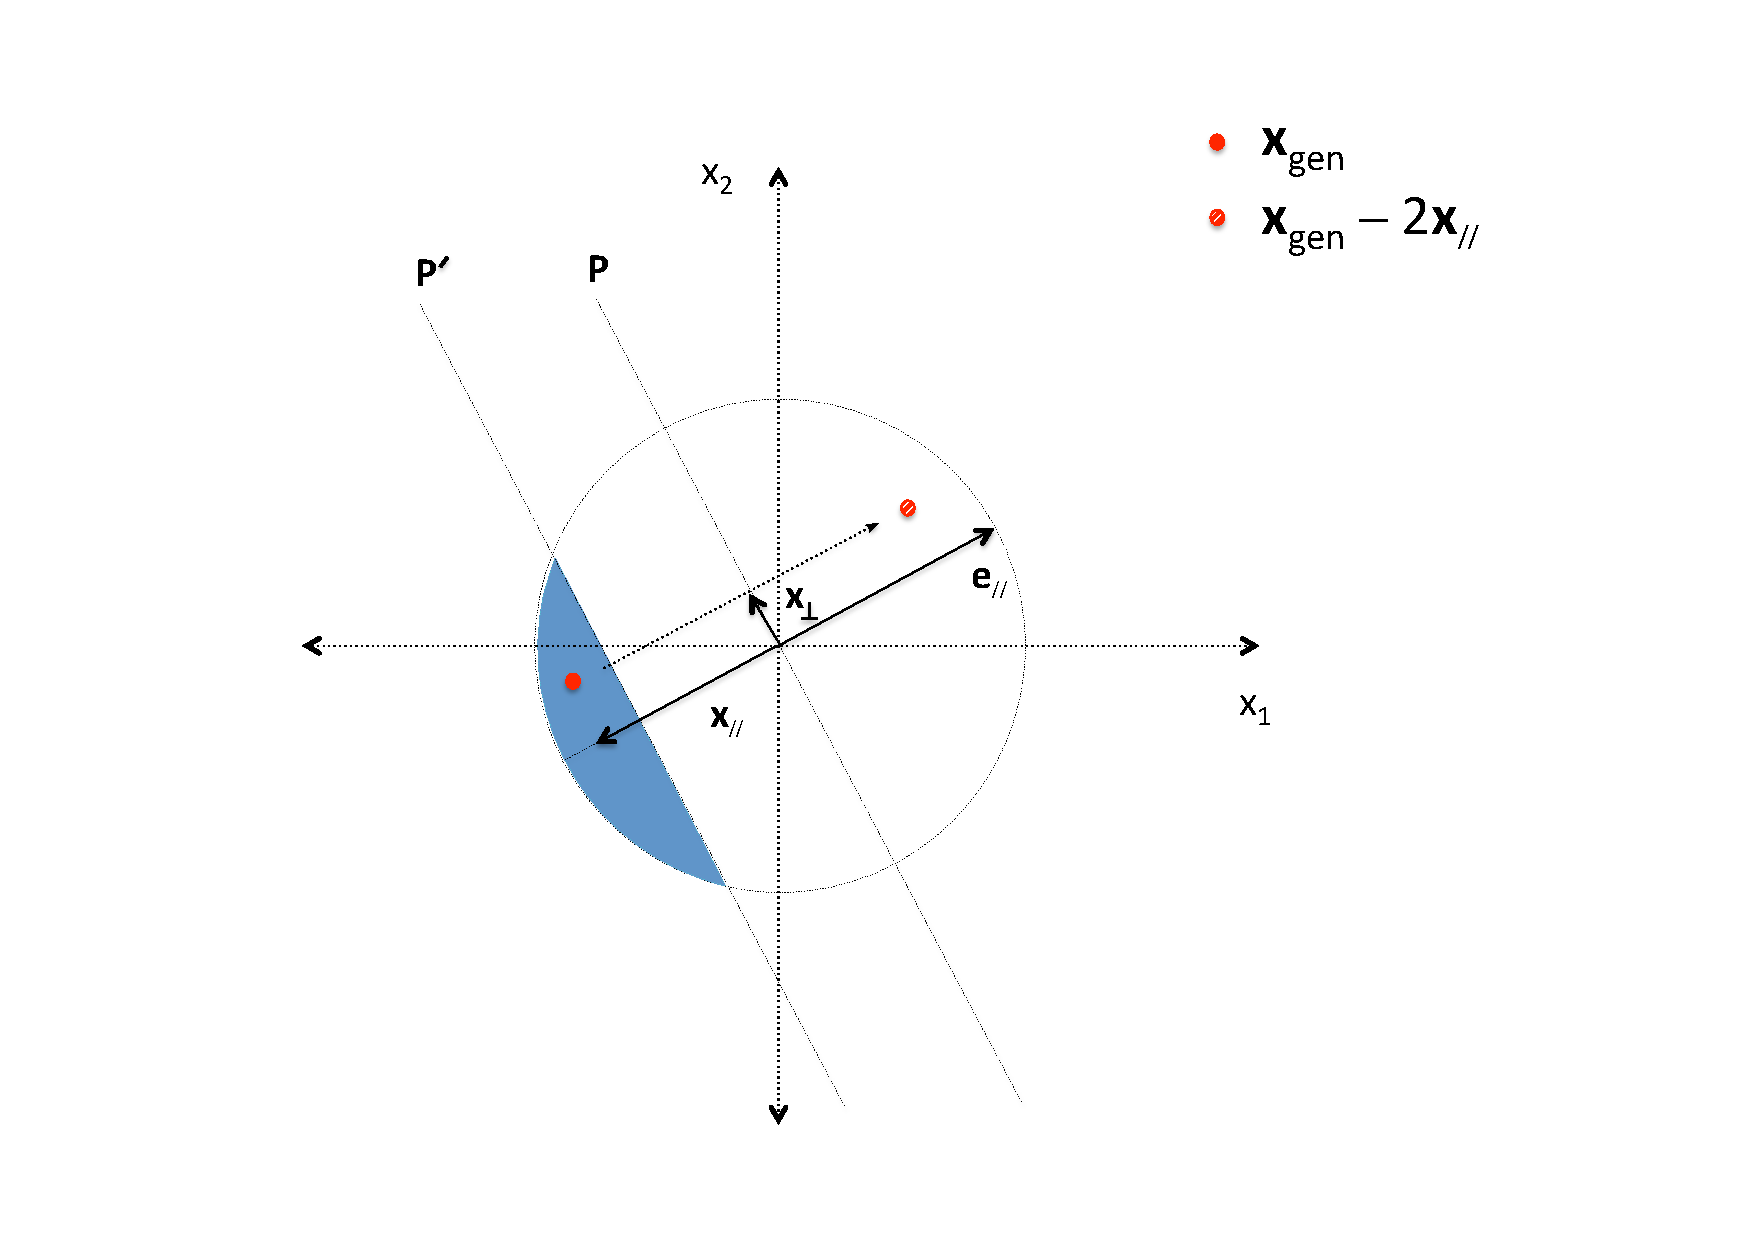
\includegraphics[width=12cm, keepaspectratio]{../resources/fig10}
		\captionbelow{An example of applying the \texttt{Truncate} transformation. The shaded area corresponds to the resulting truncated area.}
	\end{figure}

	\begin{figure}[H]
		\centering
		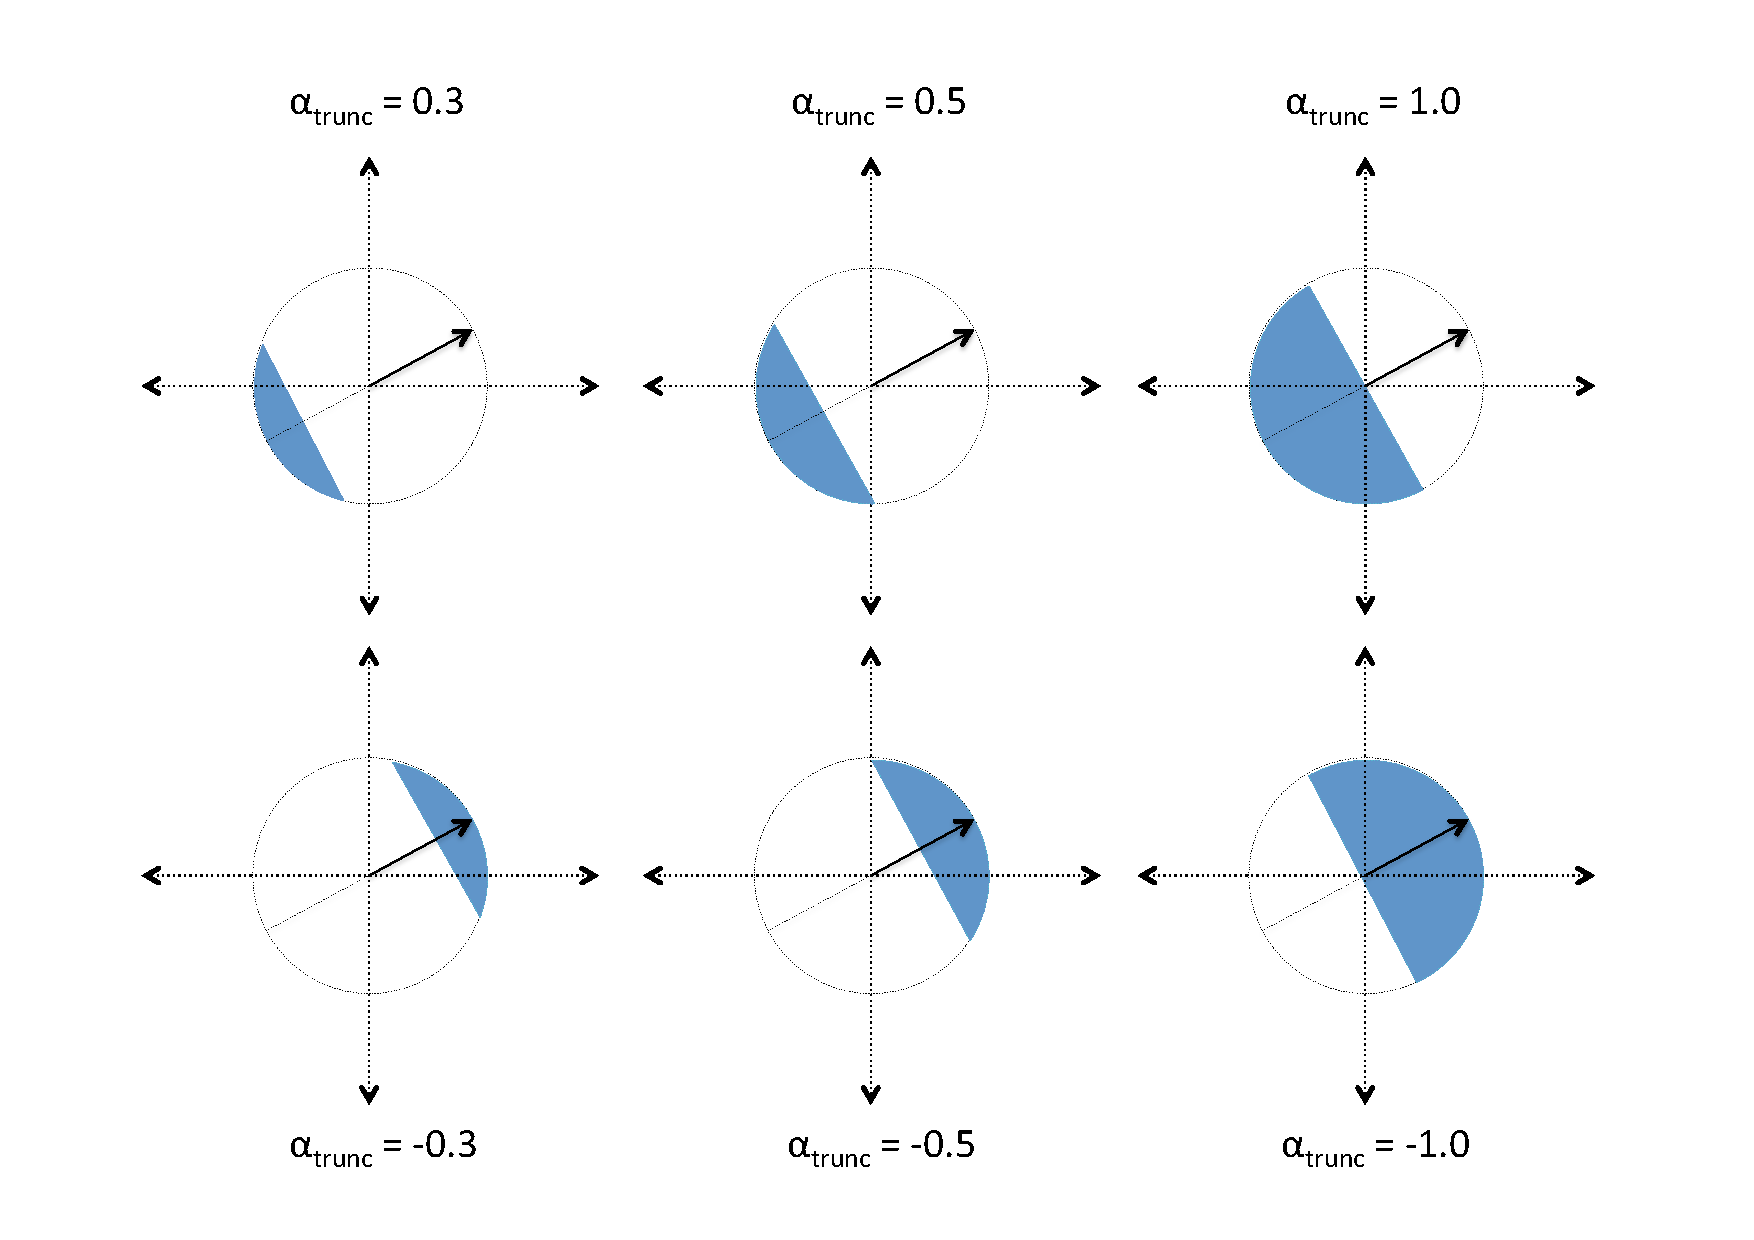
\includegraphics[width=12cm, keepaspectratio]{../resources/fig11}
		\captionbelow{Truncated areas for various values of \( \alpha_{trunc} \).}
	\end{figure}

	\item This step describes a transformation that corresponds to the deformation of the hyper-sphere in to a hyper-spheroid. More concretely, the point \( \textbf{x}_{gen} \) is moved to a perpendicular direction to the unit vector \( \textbf{e}_{\scriptscriptstyle//} \), towards the parallel to \( \textbf{e}_{\scriptscriptstyle//} \) diameter. This mapping is controlled by the \( \alpha_{def} \) hyper-parameter and from equation \eqref{eqn:deform} changes linearly with it. Therefore any point located at the surface of the hyper-sphere will remain to the surface of the new boundary while all the axes, except the one defined by the \( \textbf{e}_{\scriptscriptstyle//} \) unit vector, rescale by the factor \( \alpha_{def} \). This effectively corresponds to the formation of a hyper-spheroid boundary with symmetry axis at the \( \textbf{e}_{\scriptscriptstyle//} \) direction. Similarly to the truncation, the deformation transformation further modifies the initially uniform probability distribution. Fig. 12 presents a deformation of the unit hyper-sphere and the resulting mapping of the \( \textbf{x}_{gen} \) point. Fig. 13 shows the effect of increasing the \( \alpha_{def} \) values on the hyper-sphere deformation.

	\begin{figure}[H]
		\centering
		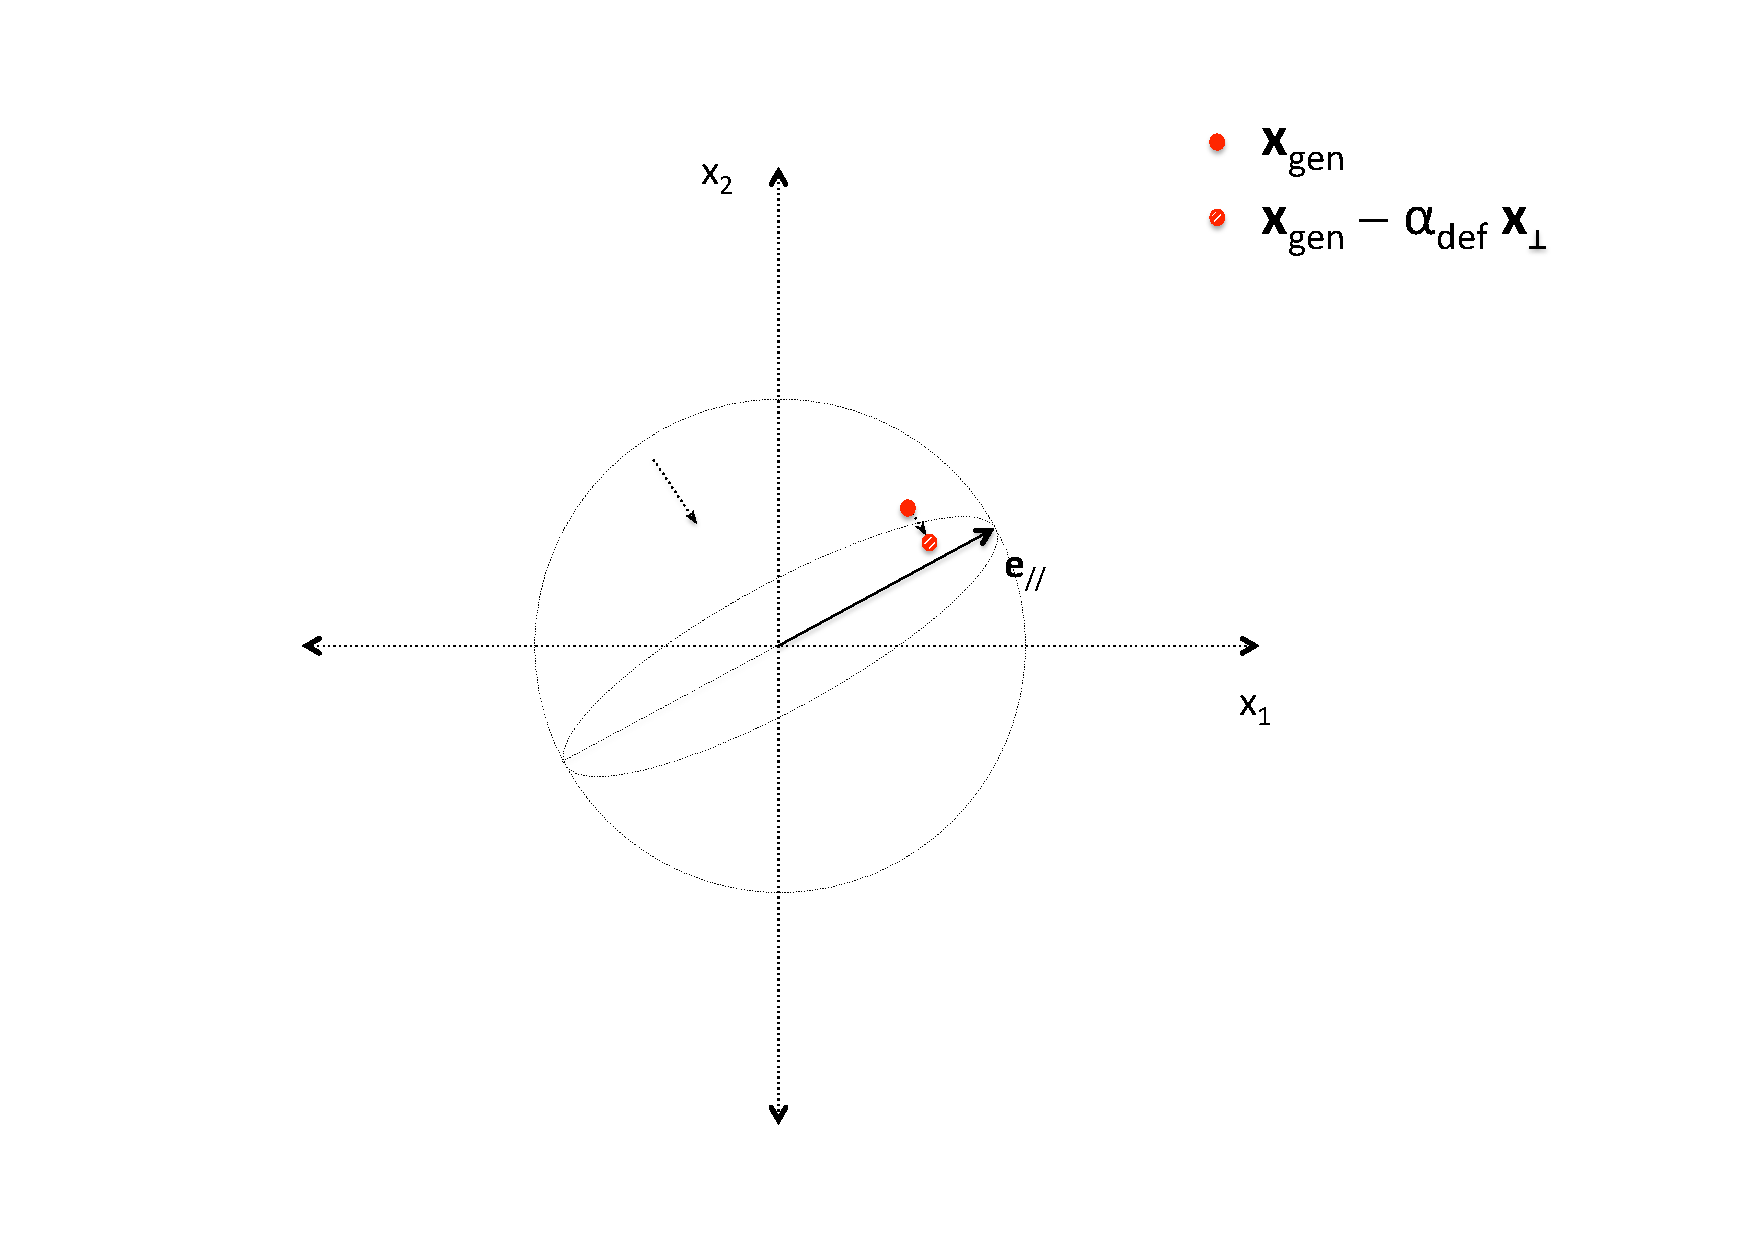
\includegraphics[width=12cm, keepaspectratio]{../resources/fig12}
		\captionbelow{The transformation \texttt{Deform} is applied and the generated point is mapped to a new point towards the diameter of the hyper-sphere.}
	\end{figure}
	
	\begin{figure}[H]
		\centering
		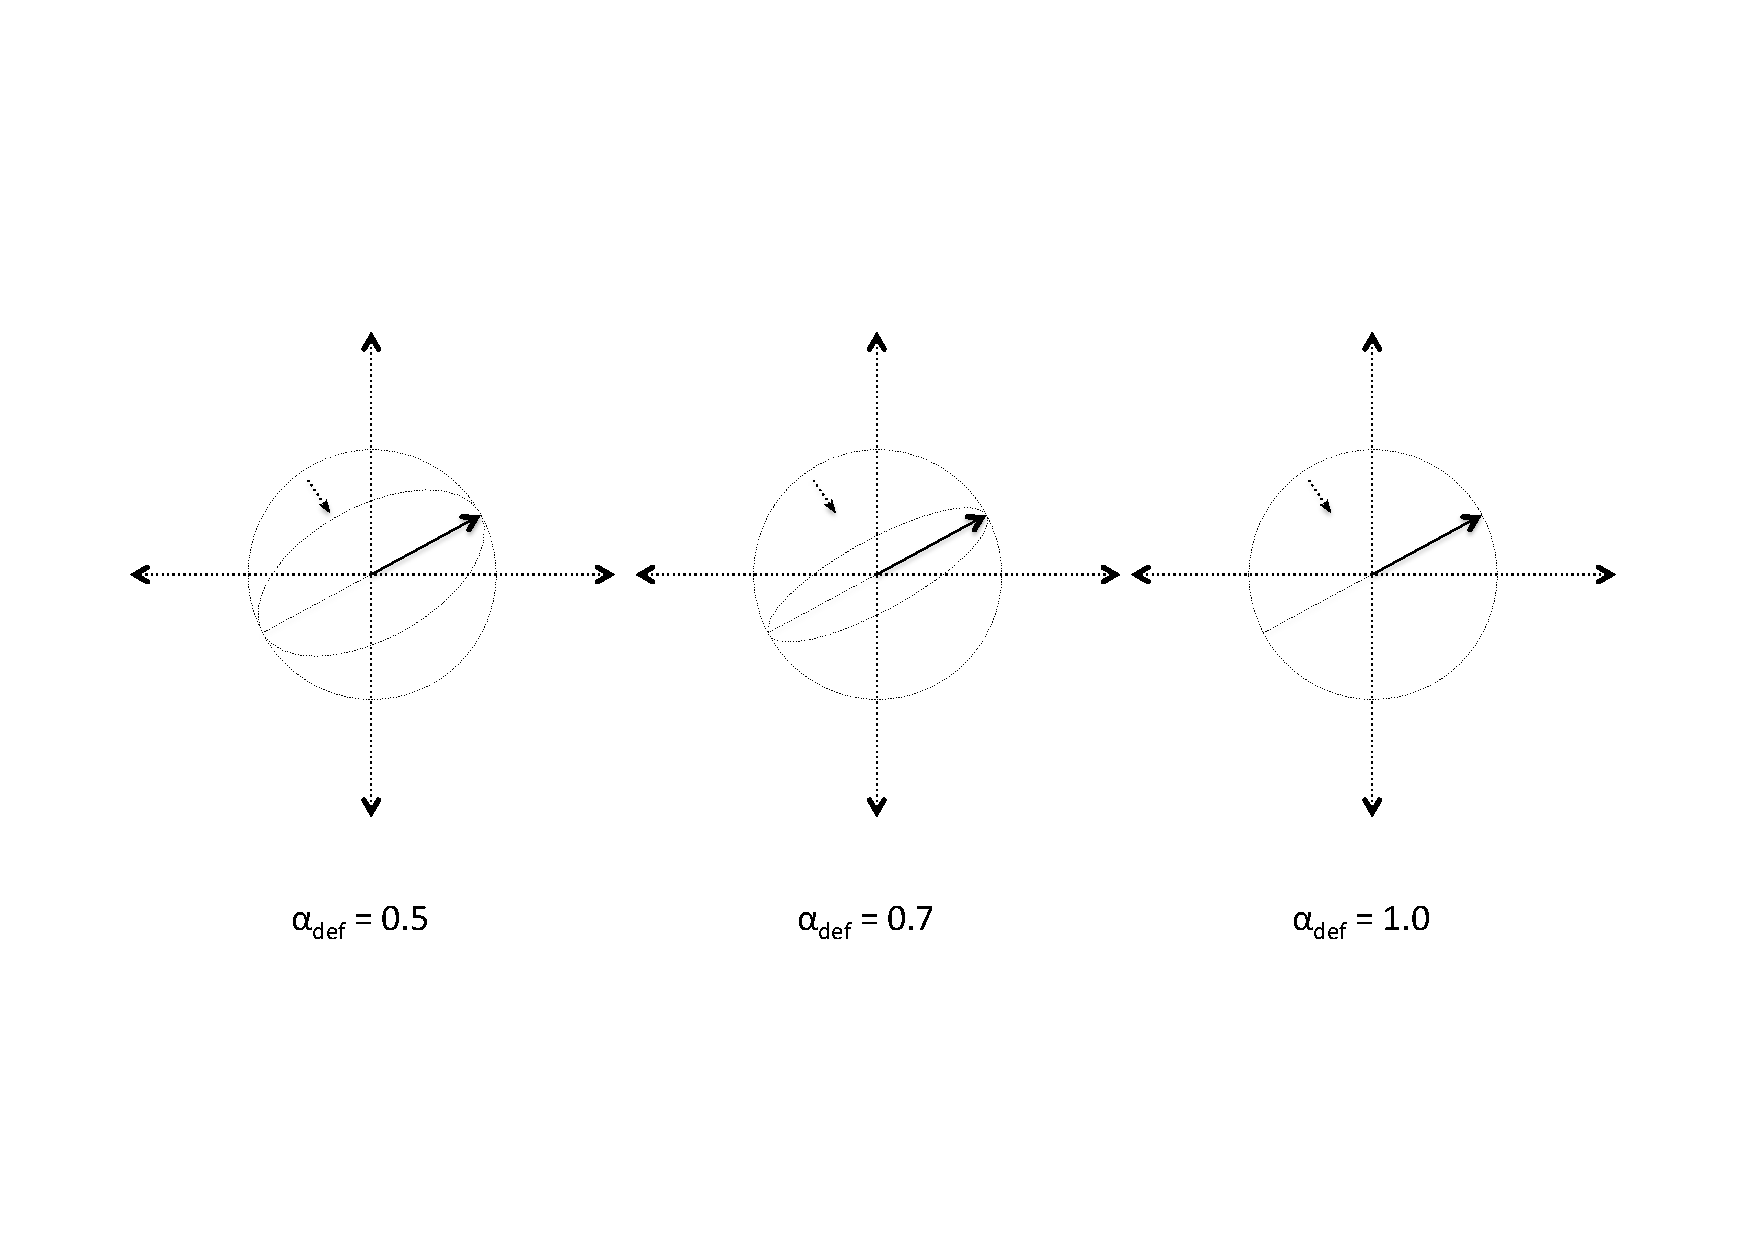
\includegraphics[width=12cm, keepaspectratio]{../resources/fig13}
		\captionbelow{The effect of increasing \( \alpha_{def} \) on the hypersphere deformation. The last case corresponds to a line segment.}
	\end{figure}

	\item The final step of the algorithm is the translation of the generated point by the \( \textbf{x}_{center} \) vector and the rescaling by the value of the radius \( R \). The combined result of this two transformations is described in equation \eqref{eqn:translate}. Fig. 14 and fig. 15 show the resulting boundaries of the permissible data generation area as well as a random generated point \( \textbf{x}_{center} \), of the two different scenarios presented in fig. 7 and fig. 8, after the application of truncation, deformation and translation.

	\begin{figure}[H]
		\centering
		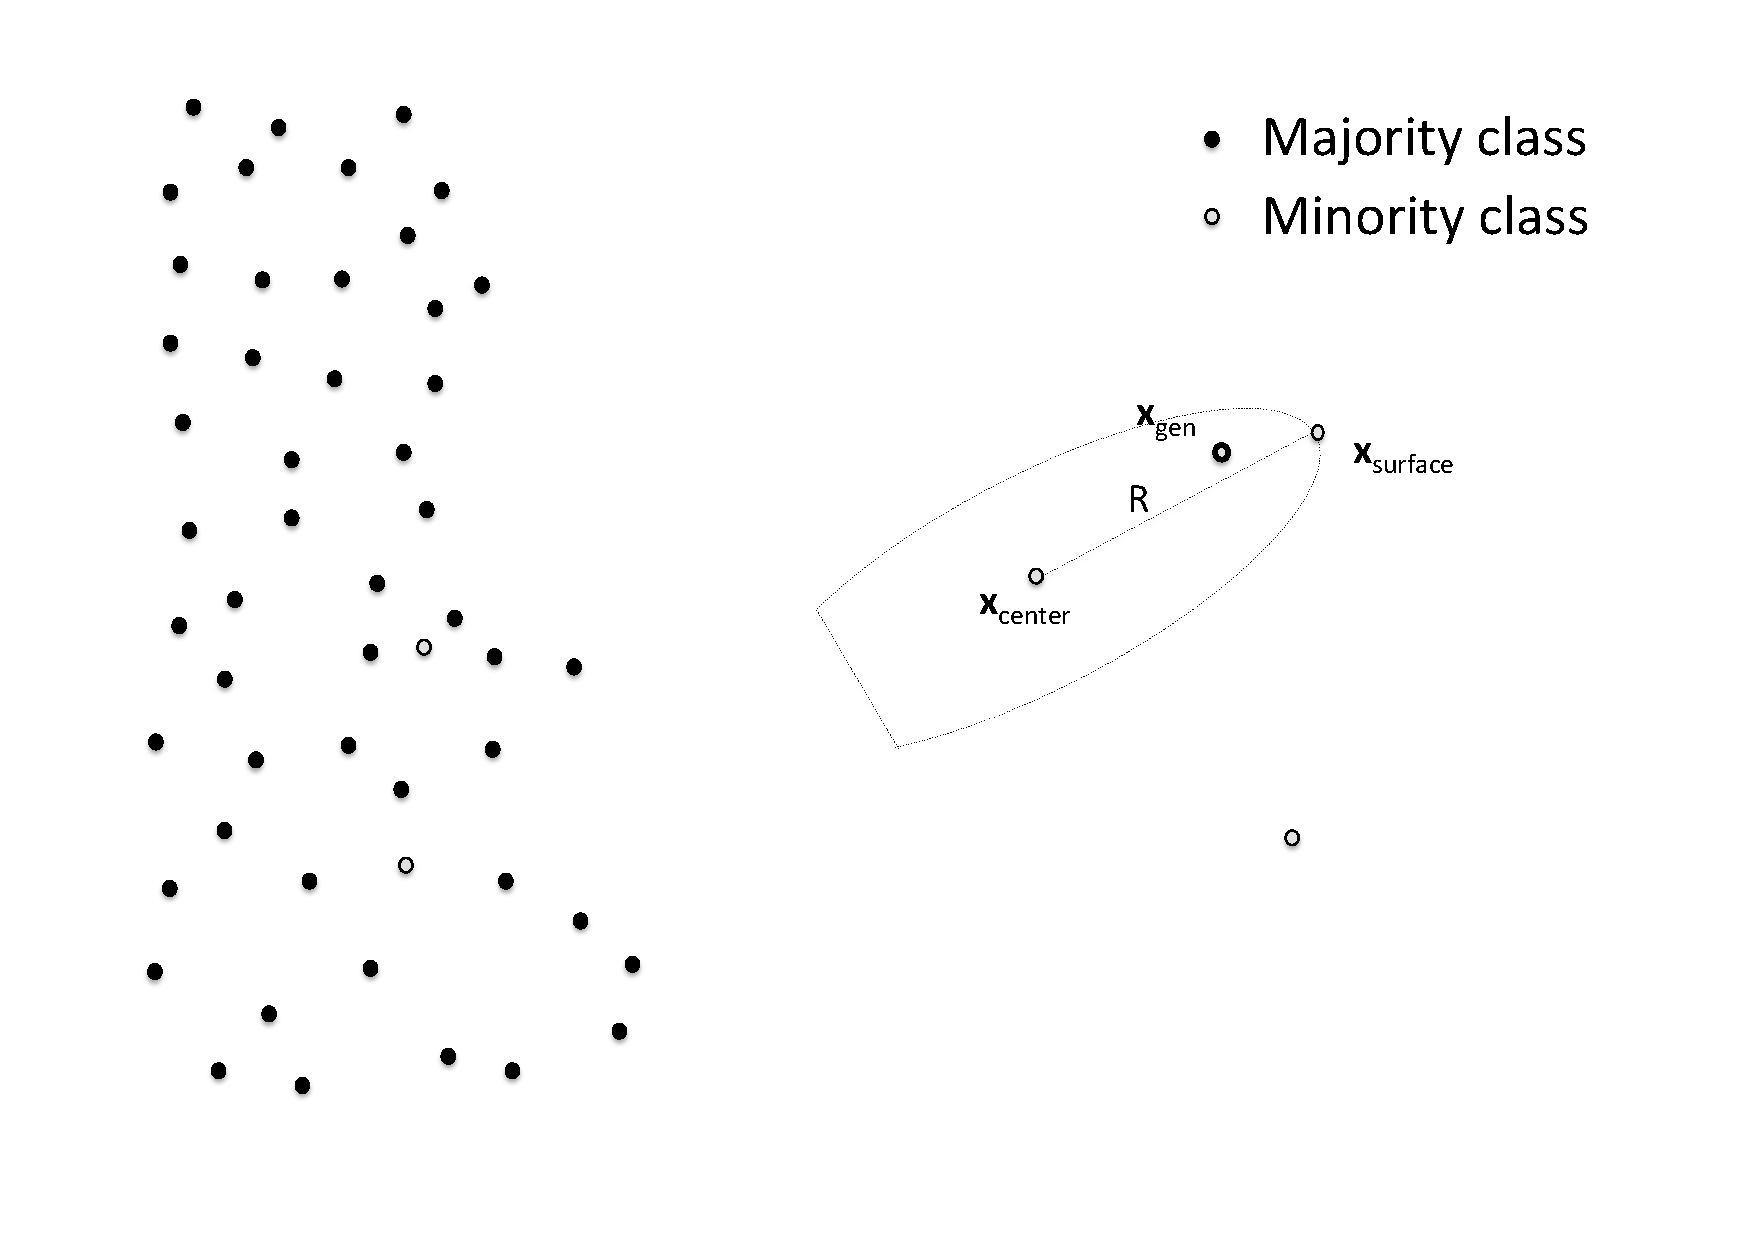
\includegraphics[width=12cm, keepaspectratio]{../resources/fig14}
		\captionbelow{Boundaries of permissible data generation area  for the scenario of Fig 7.}
	\end{figure}
	
	\begin{figure}[H]
		\centering
		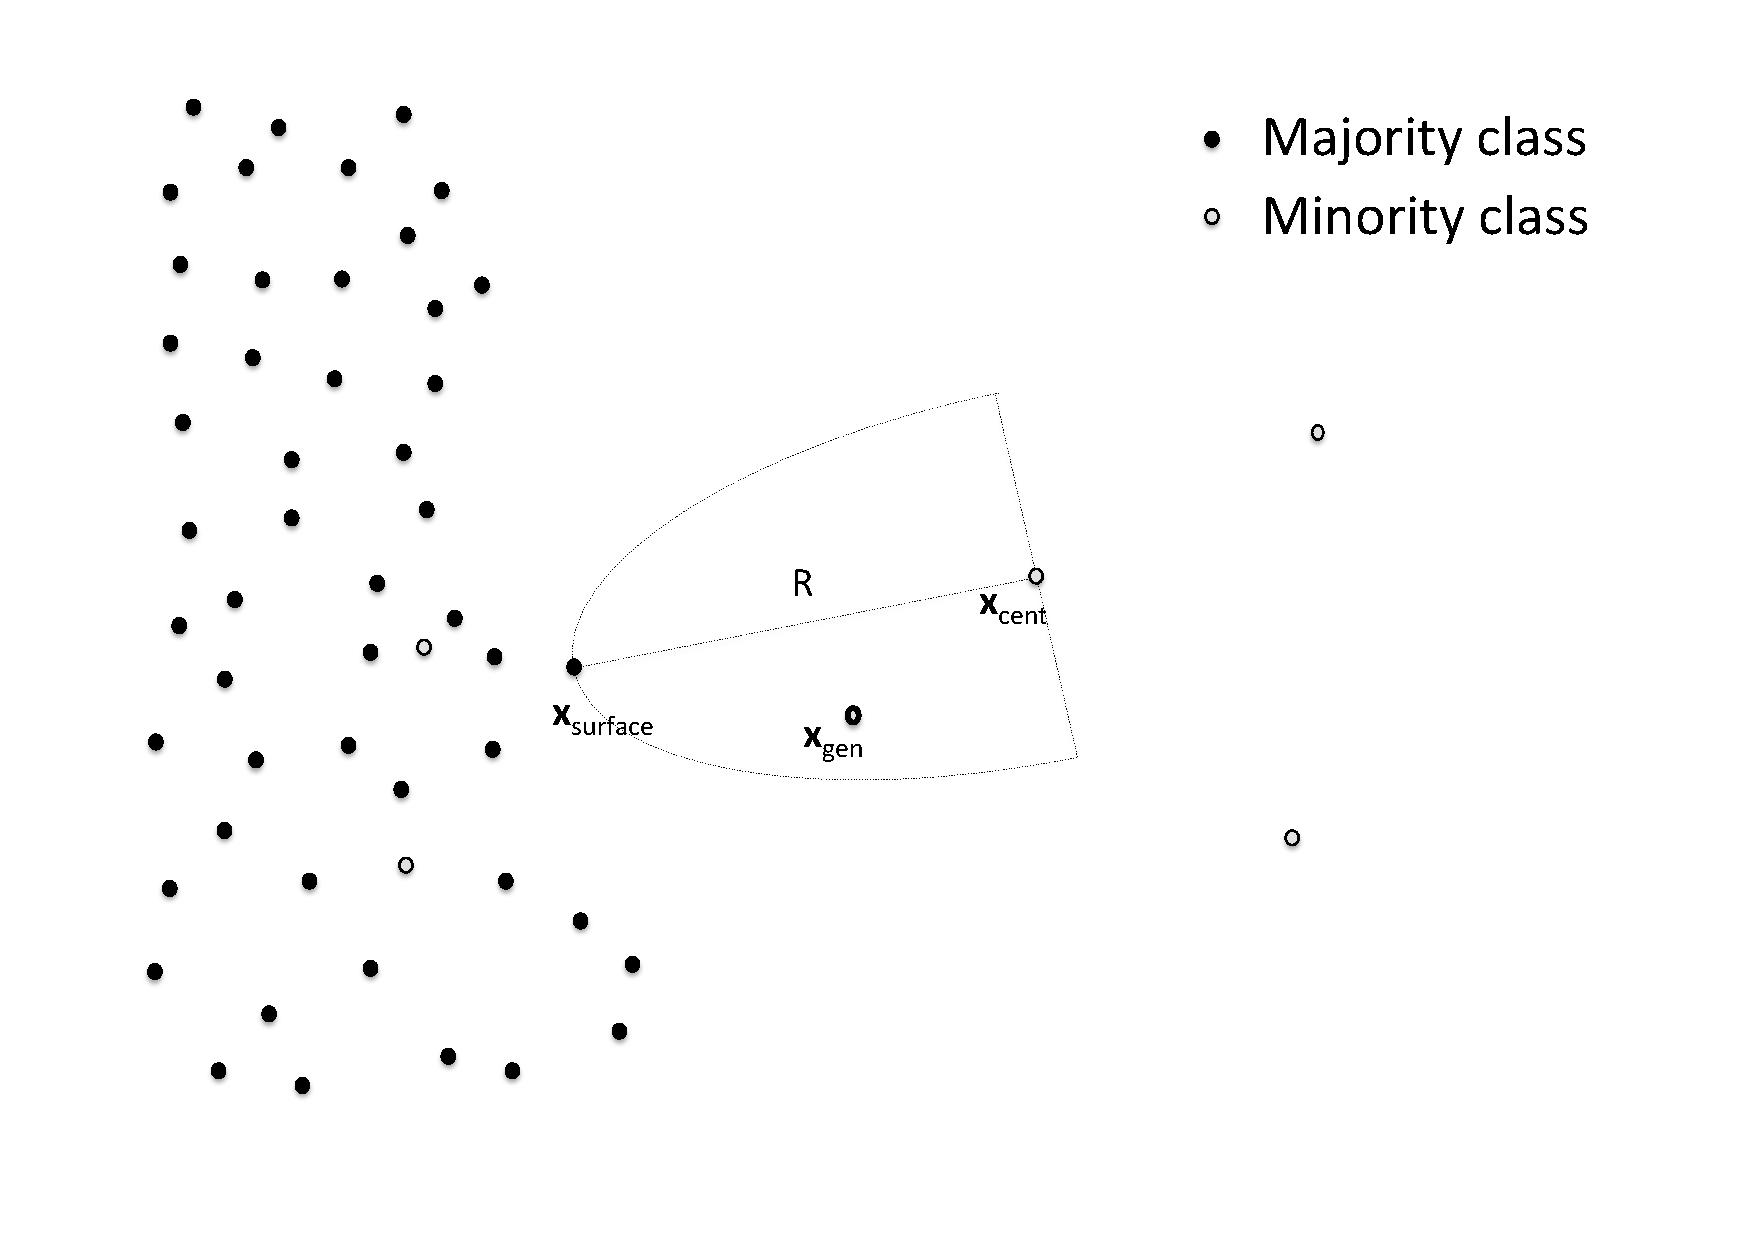
\includegraphics[width=12cm, keepaspectratio]{../resources/fig15}
		\captionbelow{Boundaries of permissible data generation area for the scenario of Fig 8.}
	\end{figure}

\end{enumerate}

\section{Research methodology and experimental results}

This section describes the evaluation process of G-SMOTE using a variety of classifiers, datasets and metrics. An extensive performance comparison of G-SMOTE to Random Oversampling and SMOTE is presented, using a cross validation procedure where the significance of the results is verified through appropriate statistical tests. Additionally, an analysis of the G-SMOTE hyper-parameters is included as well as guidelines for their tuning relative to the IR of the dataset.

\subsection{Experimental data}

In order to test the performance of G-SMOTE we used the following imbalanced datasets:

\begin{itemize}
	
	\renewcommand\labelitemi{--}

	\item UCI Machine Learning Repository, 13 datasets.

	\item KEEL repository, 13 datasets.

	\item Simulated data based on variations of the "MANDELON" dataset \cite{Guyon2003}, 2 datasets.

\end{itemize}

 Furthermore, additional datasets with even higher imbalance ratios were generated, by randomly undersampling the minority classes of the aforementioned datasets. For each one of them, its initial IR was multiplied by a factor of 2 and 3 but the resulting dataset was used for the experiments only if the total number of minority samples was not less than 15. Table 1 shows a summary of the final 69 data sets that can be found at \url{https://github.com/IMS-ML-Lab/research-showcase/tree/master/data/binary-numerical-imbalanced}. The multiplication factor is appended in parentheses to the dataset's names while the table is sorted by ascending IR:

\pgfplotstabletypeset[
begin table=\begin{longtable},
end table=\end{longtable},
col sep=comma,
header=true,
columns={Dataset name,Features,Instances,Minority instances,Majority instances,Imbalance Ratio},
columns/Dataset name/.style={column type=l,string type},
columns/Features/.style={fixed,fixed zerofill,precision=0,column type=r},
columns/Instances/.style={fixed,fixed zerofill,precision=0,column type=r},
columns/Minority instances/.style={fixed,fixed zerofill,precision=0,column type=r},
columns/Majority instances/.style={fixed,fixed zerofill,precision=0,column type=r},
columns/Imbalance Ratio/.style={fixed,fixed zerofill,precision=2,column type=r},
every head row/.style={before row=\toprule, after row=\midrule\endhead},
every last row/.style={after row=\bottomrule \caption{Description of the datasets.}}
]
{../resources/imbalanced_datasets_summary.csv}

\subsection{Evaluation measures}

Various assessment metrics can be used to evaluate a classifier's performance. However, not all of them are suitable for imbalanced datasets \cite{He2009}. The most common metric for binary classification problems is accuracy defined as the ratio of correct predictions for both of the classes over the total number of predictions:

$$Accuracy = \frac{TP + TN}{TP +TN + FP + FN}$$

where \(TP / TN\) and \(FP / FN\) are the true positives/negatives and false positives/negatives, respectively. When the class distribution is imbalanced, assuming that the minority class is identified as the \(P\) label, the contribution of \(TP\) and \(FP\) to the above formula might be negligible, i.e. accuracy is mainly determined by the majority class contribution. Based on this, the selected evaluation metrics of the experimental procedure are following:

\begin{itemize}
	
	\renewcommand\labelitemi{--}
	
	\item Area Under the ROC Curve (AUC):
	
	ROC curve results from varying the decision threshold and plotting the true positive rate against the false positive rate.
	
	\item F-score:
	
	It is defined as the harmonic mean of \(Precision\) and \(Recall\), where \(Precision = \frac{TP}{TP + FP}\) and \(Recall = \frac{TP}{TP + FN}\).
	
	\item G-mean:
	
	It is defined as the geometric mean of \(Sensitivity\) and \(Specificity\), where \(Sensitivity = \frac{TP}{TP + FN}\) and \(Specificity = \frac{TN}{TN + FP}\).
	
\end{itemize}

\subsection{Machine learning algorithms}

The main objective of the paper is to compare G-SMOTE and SMOTE algorithms. Therefore their performance was evaluated on the aforementioned 69 datasets. Additionally, the use of unmodified data (NO OVERSAMPLING) and random oversampling (RANDOM OVERSAMPLING) were included as a baseline methods.

For the evaluation of the oversampling methods the following 4 classifiers were used: Logistic Regression (LR) \cite{McCullagh1989}, K-Nearest Neighbors (KNN) \cite{Cover1967}, Decision Tree (DT) \cite{Salzberg1994} and Gradient Boosting (GBC) \cite{Friedman2001}.

The implementation of the classifiers and standard oversampling algorithms was based on the Python libraries Scikit-Learn \cite{Pedregosa2011} and Imbalanced-Learn \cite{Lemaitre2016}.

\subsection{Experimental results}

\subsubsection{Experimental procedure}

In order to evaluate the performance of each combination of oversampler and classifier, \( n \)-fold cross validation was applied with \( n = 5 \). Let \(D\) one of the datasets. Before starting the training of the classifier, in each stage \(i \in \{1, 2 ,... , n \} \) of the \( n \)-fold cross validation procedure, synthetic data \( T_{g, i} \) were generated from the oversampler based on the training data \(T_{i} \) of the \( n - 1 \) folds such that the resulting \(T_{g, i} \cup T_{i} \) training set becomes perfectly balanced. This enhanced training set in turn was used to train the classifier. The performance evaluation of the classifiers was done on the validation data \( V_{i} \) of the remaining fold, where \(V_{i} \cup T_{i} = D \) and \(V_{i} \cap T_{i} = \emptyset \).

A variety of hyper-parameters were used for the the oversamplers and classifiers. For SMOTE the optimal value of \( k \) nearest neighbors was selected as \( k \in \{ 3, 5 \} \) while for G-SMOTE a hyper-parameter grid was generated from the Cartesian product of the three different selection strategies, the number of nearest neighbors \(k \in \{ 3, 5 \} \), the truncation factor \( \alpha_{trunc} \in \{ -1.0, -0.5, 0.0, 0.25, 0.5, 0.75 , 1.0 \} \) and the deformation factor \( \alpha_{def} \in \{ 0.0, 0.2, 0.4, 0.5, 0.6, 0.8, 1.0 \} \). As far the classifiers are concerned, the number of nearest neighbors for KNN was selected as \( k \in \{ 3, 5 \} \),  the max depth for DT was selected as \( \textit{max depth} \in \{ 3, 6 \} \) while GBC hyper-parameter grid included the four combinations resulting from the Cartesian product of  \textit{max depth} \( \in \{ 3 , 6 \} \) and \textit{number of estimators} \( \in \{50, 100\} \).

Using the above hyper-parameters, the highest cross validation score for each combination of datasets, classifiers, oversamplers and evaluation metrics was reported. The experimental procedure was repeated 3 times and the reported results include the average values between the experiments. A ranking score was assigned to each oversampling method with the best and worst performing methods receiving scores equal to 1 and 4, respectively. We apply the Friedman test to confirm the statistical significance of the ranking results of the experiments \cite{Guyon2003}. The Friedman test is used to detect differences for a set of experimental attempts when normality assumption may not hold. In this case the null hypothesis represents the situation in which the classifiers show an identical performance, in terms of their mean ranking, independently of the oversampling method and performance metric used.  Additionally, we apply the Holm’s test, using G-SMOTE as the control method \cite{Guyon2003}. The Holm’s test is a non-parametric version of the t-test, where the null hypothesis is whether the proposed G-SMOTE algorithm outperforms the other methods as the control method.

\subsubsection{Software implementation}

As it was mentioned above, the implementation of the experimental procedure is based on the Python programming language and Scikit-Learn/Imbalanced-Learn libraries. Specifically, the function that prepares and runs any comparative experiment can be found at \url{https://github.com/georgedouzas/scikit-learn-extensions/blob/master/sklearnext/tools/imbalanced_analysis.py}, while the G-SMOTE implementation is available at \url{https://github.com/georgedouzas/scikit-learn-extensions/blob/master/sklearnext/over_sampling/geometric_smote.py}. Being fully integrated with the Scikit-Learn ecosystem they can be adjusted and used for a variety of custom comparative studies. The experiments reported in this paper as well as the analysis of their results are reproducible using the scripts provided at \url{https://github.com/IMS-ML-Lab/publications/tree/master/scripts/gsmote-journal}.

\subsubsection{Comparative presentation}

The mean cross validation scores across datasets for each combination of classifiers, metrics and oversamplers are presented in Table 2:

\pgfplotstabletypeset[
begin table=\begin{longtable},
	end table=\end{longtable},
col sep=comma,
header=true,
columns={Classifier,Metric,NO OVERSAMPLING,RANDOM OVERSAMPLING,SMOTE,G-SMOTE},
columns/Classifier/.style={column type=l,string type},
columns/Metric/.style={column type=l,string type},
columns/NO OVERSAMPLING/.style={fixed,fixed zerofill,precision=3,column type=r},
columns/RANDOM OVERSAMPLING/.style={fixed,fixed zerofill,precision=3,column type=r},
columns/SMOTE/.style={fixed,fixed zerofill,precision=3,column type=r},
columns/G-SMOTE/.style={fixed,fixed zerofill,precision=3,column type=r},
every head row/.style={before row=\toprule, after row=\midrule\endhead},
every last row/.style={after row=\bottomrule \caption{Results for mean cross validation scores of oversamplers across the datasets.}}
]
{../resources/mean_score_clf_metric_table.csv}

The table of full results is available at \url{https://github.com/IMS-ML-Lab/publications/blob/master/data/results/gsmote-journal/wide_optimal.csv}. Table 2 shows that G-SMOTE systematically performs better on average than the rest of the methods. Particularly, the percentage difference of G-SMOTE and SMOTE mean scores, relative to each classifier's score without any oversampling, is presented in Fig. 16:

\begin{figure}[H]
	\centering
	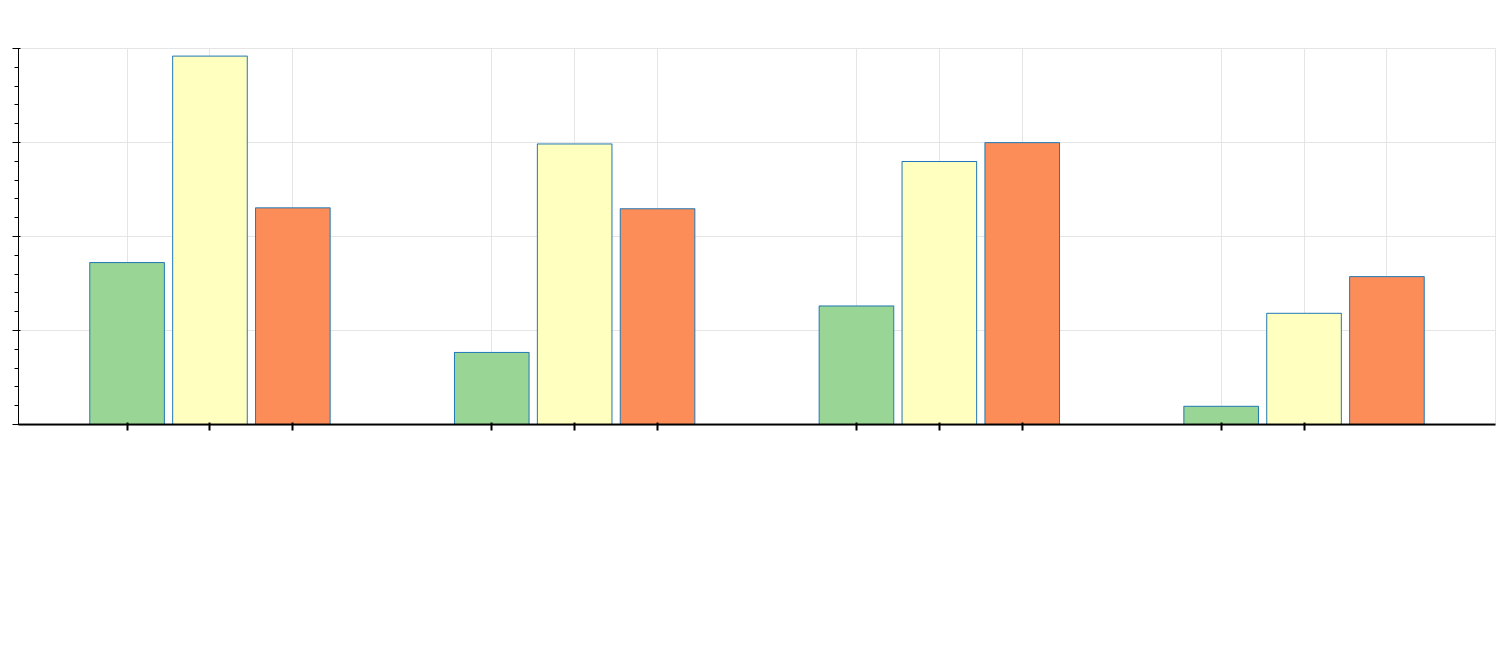
\includegraphics[width=15cm, keepaspectratio]{../resources/percentage_difference}
	\captionbelow{Percentage difference of G-SMOTE and SMOTE, relative to the score of each classifier without any oversampling, calculated as \( \frac{ \text{\large{Score}} [\text{\tiny{G-SMOTE}}] -\text{\large{Score}} [\text{\tiny{SMOTE}}] } { \text{\large{Score}} [\text{\tiny{NO OVERSAMPLING}}] } \times 100\% \).}
\end{figure}

As explained in section 5.4 a ranking score in the range 1 to 4 is assigned to each oversampler. Then the mean ranking of the oversampling methods across the data sets for each combination of a classifier and evaluation metric is presented in Table 3:

\pgfplotstabletypeset[
begin table=\begin{longtable},
end table=\end{longtable},
col sep=comma,
header=true,
columns={Classifier,Metric,NO OVERSAMPLING,RANDOM OVERSAMPLING,SMOTE,G-SMOTE},
columns/Classifier/.style={column type=l,string type},
columns/Metric/.style={column type=l,string type},
columns/NO OVERSAMPLING/.style={fixed,fixed zerofill,precision=3,column type=r},
columns/RANDOM OVERSAMPLING/.style={fixed,fixed zerofill,precision=3,column type=r},
columns/SMOTE/.style={fixed,fixed zerofill,precision=3,column type=r},
columns/G-SMOTE/.style={fixed,fixed zerofill,precision=3,column type=r},
every head row/.style={before row=\toprule, after row=\midrule\endhead},
every last row/.style={after row=\bottomrule \caption{Results for mean ranking of oversamplers across the datasets.}}
]
{../resources/mean_ranking_table.csv}

\subsubsection{Statistical analysis}

The results of the application of the Friedman test are shown in Table 4:

\pgfplotstabletypeset[
begin table=\begin{longtable},
	end table=\end{longtable},
col sep=comma,
header=true,
columns={Classifier,Metric,p-value,Significance},
columns/Classifier/.style={column type=l,string type},
columns/Metric/.style={column type=l,string type},
columns/p-value/.style={column type=r, zerofill, precision=1, dec sep align},
columns/Significance/.style={column type=r,string type},
every head row/.style={before row=\toprule, after row=\midrule\endhead},
every last row/.style={after row=\bottomrule \caption{Results for Friedman test.}}
]
{../resources/friedman_test_table.csv}

Therefore at a significance level of a = 0.05 the null hypothesis is rejected, i.e. the classifiers do not perform similarly in the mean rankings across the oversampling methods and evaluation metrics. Following the Friedman test, the Holm's method is applied to adjust the p-values of the paired difference test with G-SMOTE algorithm as the control method. The adjusted $\text{p-values}$ are presented in Table 5:

\pgfplotstabletypeset[
begin table=\begin{longtable},
	end table=\end{longtable},
col sep=comma,
header=true,
columns={Classifier,Metric,NO OVERSAMPLING,RANDOM OVERSAMPLING,SMOTE},
columns/Classifier/.style={column type=l,string type},
columns/Metric/.style={column type=l,string type},
columns/NO OVERSAMPLING/.style={ zerofill,precision=1,column type=r, dec sep align},
columns/RANDOM OVERSAMPLING/.style={zerofill,precision=1,column type=r, dec sep align},
columns/SMOTE/.style={zerofill,precision=1,column type=r, dec sep align},
every head row/.style={before row=\toprule, after row=\midrule\endhead},
every last row/.style={after row=\bottomrule \caption{Adjusted p-values using the Holm's method.}}
]
{../resources/adjusted_pvalues_table.csv}

Therefore, the null hypothesis of the Holm's test is rejected for all oversamplers at a significance level of a = 0.05, indicating that the proposed method outperforms all other methods.

\subsubsection{Analysis of optimal hyper-parameters}

The G-SMOTE hyper-parameters \( \alpha_{trunc} \), \( \alpha_{def} \) and \( \alpha_{sel} \) control the characteristics of the data generation process, allowing to identify some special cases that can be considered as extensions of the SMOTE algorithm with a simple geometrical interpretation. All these cases are tested during the experimental procedure and compared to the rest of the oversampling methods as well as the optimal choice of hyper-parameters for G-SMOTE. A short description is provided below:

\begin{itemize}
	
	\renewcommand\labelitemi{--}

	\item SMOTE algorithm.

	The choice of hyper-parameters that reproduces the SMOTE algorithm is \( \alpha_{def} = 1.0 \), \( \alpha_{trunc} = 1.0 \) and \( \alpha_{sel} = minority \). The first of them ensures that the initial hypersphere is deformed in to a line segment, the second truncates the half of the resulting line segment and the third chooses the SMOTE selection strategy.

	\item Majority selection SMOTE algorithm.

	The geometry of the permissible data generation areas is identical to SMOTE, thus the hyper-parameters \( \alpha_{trunc} \), \( \alpha_{def} \) are identical too, but instead of the minority selection strategy, it uses the majority one.

	\item Combined selection SMOTE algorithm.

	Similar to the previous case except the selection strategy is the combined one.

	\item Inverse SMOTE algorithm.

	Similar to case 1 except the truncation of the line segment occurs at the opposite direction. This requires a modification of \( \alpha_{trunc} \) value to \( \alpha_{trunc} = -1.0 \).

	\item Hyper-sphere SMOTE algorithm.

	This extension of SMOTE generates artificial data inside a hyper-ball with center a minority class instance and a radius equal to the distance of it with one of its minority class \( k \) nearest neighbors. The choice of hyper-parameters in this case is \( \alpha_{def} = 0.0 \), \( \alpha_{trunc} = 0.0 \) and \( \alpha_{sel} = minority \).

	\item Half hyper-sphere SMOTE algorithm.

	Similar to the previous case except only half of the hyper-sphere is used as a permissible data generation area. This requires \( \alpha_{trunc} = 1.0 \).

\end{itemize}

As it was described in section 5.4.1, the generated hyper-parameter space for G-SMOTE was 4-dimensional and included the following dimensions:

\begin{itemize}
	
	\renewcommand\labelitemi{--}

	\item Selection strategy.

	\item Truncation factor.

	\item Deformation factor.

	\item Number of nearest neighbors.

\end{itemize}

 The first three of them, called geometric hyper-parameters, adjust the geometric configuration of G-SMOTE. Their percentage contribution to the optimal hyper-parameter settings is shown in Fig. 17:

\begin{figure}[H]
	\centering
	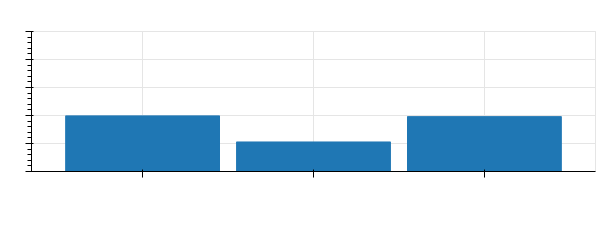
\includegraphics[width=14cm, keepaspectratio]{../resources/selection_strategy}
\end{figure}

\begin{figure}[H]
	\centering
	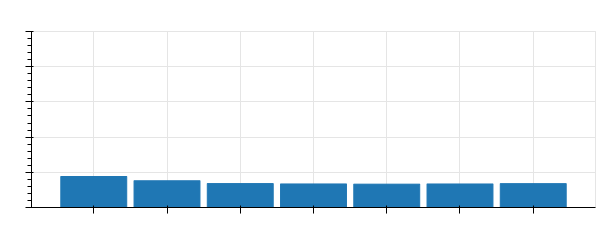
\includegraphics[width=14cm, keepaspectratio]{../resources/truncation_factor}
\end{figure}

\begin{figure}[H]
	\centering
	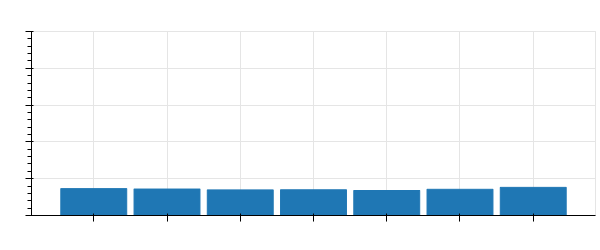
\includegraphics[width=14cm, keepaspectratio]{../resources/deformation_factor}
	\captionbelow{Percentage contribution of geometric hyper-parameters to the optimal configurations of experiments.}
\end{figure}

The majority of optimal values for the \( \alpha_{sel} \) hyper-parameter are split between the minority and combined selection strategies, while the majority selection strategy has a lower but not negligible contribution. On the other hand, the distribution of optimal values for the \( \alpha_{trunc} \) and \( \alpha_{def} \) hyper-parameters is approximately uniform.

The number of points in the hyper-parameter subspace \( H_{sub} \), formed only by the geometric hyper-parameters is equal to $N(\{ minority, majority, combined \}) \times N(\{ -1.0, -0.5, 0.0, 0.25, 0.5, 0.75 , 1.0 \}) \times N(\{ 0.0, 0.2, 0.4, 0.5, 0.6, 0.8, 1.0 \}) = 147$. Therefore a ranking score between 1 to 147 can be assigned to each point of \( H_{sub} \), by counting the number of times it appears as the optimal configuration across all the experiments. Fig. 18 shows the ranking of the above special cases:

\begin{figure}[H]
	\centering
	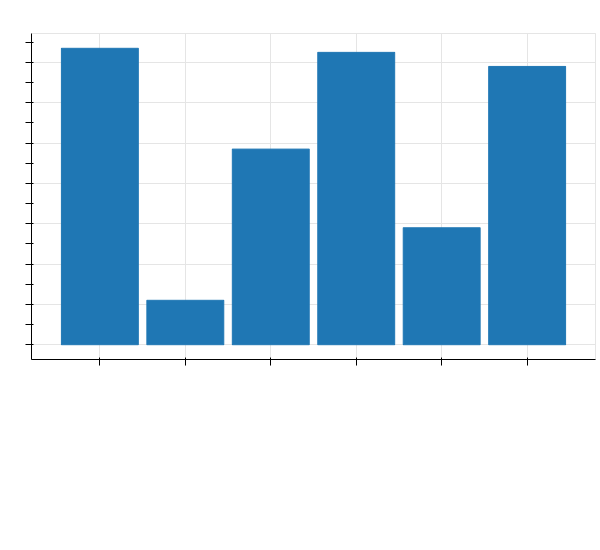
\includegraphics[width=14cm, keepaspectratio]{../resources/cases_rank}
	\captionbelow{Frequency ranking of the 6 special cases.}
\end{figure}

SMOTE, inverse SMOTE and half hyper-sphere SMOTE, as described above, represent the configurations with the highest frequency ranking among the 6 special cases. It is important to notice that Fig. 18 shows only  6 of the 147 possible configurations. On the other hand, Fig. 17 shows that there is an approximately uniform distribution of the optimal hyper-parameters values, meaning that all the points of the generated hyper-parameter space are important. Also a non-intuitive observation is that inverse SMOTE appears to be an effective approach having a high ranking score.

Finally, an analysis of the relation between optimal hyper-parameters and IR shows that lower \( \alpha_{def} \) values should be selected as the dataset's IR increases. An explanation for this finding is the following: The SMOTE data generation mechanism, which corresponds to high \( \alpha_{def} \) values, for highly imbalanced datasets   creates nearly duplicate examples.  Therefore when low \( \alpha_{def} \) values are selected, the variety of generated samples is increased.

\subsection{Discussion}

In this paper we presented G-SMOTE, a new oversampling algorithm, that extends the SMOTE data generation mechanism. G-SMOTE selects a safe radius around each minority class instance and generates artificial data within a (truncated) hyper-spheroid. G-SMOTE performance was evaluated on 69 datasets with different imbalance ratios and compared to no oversampling, Random Oversampling and SMOTE, using Logistic Regression, K-Nearest Neighbors, Decision Tree and Gradient Boosting Machine as classifiers.

The results show that G-SMOTE performs significantly better compared to the other methods. The explanation for this improvement in performance relates to the ability of G-SMOTE to generate artificial data in safe areas of the input space, while, at the same time, aggressively increasing the diversity of the generated instances. G-SMOTE parametrizes efficiently the data generation process and adapts to the special characteristics of each imbalanced dataset. We make available an implementation of G-SMOTE at \url{https://github.com/georgedouzas/scikit-learn-extensions/blob/master/sklearnext/over_sampling/geometric_smote.py}.

G-SMOTE can be a useful tool for researchers and practitioners since it results in the generation of high quality artificial data and only requires the tuning of a small number of parameters.

\bibliography{references}
\bibliographystyle{apalike}

\end{document}
